\documentclass[a4paper,12pt,twocolumn]{article}
\usepackage[dvipsnames]{xcolor}
\usepackage{tikz}
\usetikzlibrary{calc}
\usepackage{anyfontsize}
\usepackage{sectsty}
\usepackage[spanish]{babel}
\usepackage[utf8]{inputenc}
\usepackage[T1]{fontenc}
\usepackage[left=2.54cm,right=2.54cm,top=2.54cm,bottom=2.54cm, headheight=28pt]{geometry}
\usepackage{amsmath}
\usepackage{amssymb}
\usepackage{amsthm}
\usepackage{amsfonts}
\usepackage{mathtools}
\usepackage{hyperref}
\usepackage{graphicx}
\usepackage{fancyhdr}
\usepackage{multicol}
\usepackage{balance}
\usepackage[font=footnotesize]{caption}
\usepackage[export]{adjustbox}
\usepackage{subcaption}
\usepackage{wrapfig}
\usepackage{float}
\usepackage{url}
\usepackage{listings}
\usepackage{enumitem}
\usepackage{gensymb}
\usepackage{setspace}
\usepackage{chessboard}
\usepackage{array}
\usepackage{extramarks}
\usepackage{xurl}
\newcolumntype{L}[1]{>{\raggedright\arraybackslash}p{#1}}
\usepackage[backend=bibtex, style=numeric]{biblatex}
\addbibresource{referencias.bib}

\hypersetup{
	colorlinks=true,
	linkcolor=AirForceBlue,
	filecolor=green,
	citecolor = blue,
	urlcolor=blue,
}

\definecolor{skyblue}{RGB}{122,177,226}
\definecolor{daphne}{RGB}{51,118,185}
\definecolor{AirForceBlue}{RGB}{21,58,89}
\definecolor{midnight}{RGB}{18,34,62}
\setlength{\parindent}{0pt}

\pagestyle{fancy}
\fancyhf{}
\lhead{\scriptsize \nouppercase{\firstleftmark}}
\rhead{\scriptsize \nouppercase{\firstrightmark}}
\cfoot{\thepage}
\renewcommand{\headrulewidth}{1pt}

\lstdefinestyle{pythonish}{
	basicstyle=\ttfamily\small,
	language=python,
	numberstyle=\tiny\color{gray},
	numbers=left,
	stepnumber=1,
	numbersep=10pt,
	tabsize=4,
	showspaces=false,
	showstringspaces=false,
	breaklines=true,
	frame=single,
	rulecolor=\color{black},
	showtabs=false,
	captionpos=b,
	keywordstyle=\color{blue},
	commentstyle=\color[HTML]{8a8b91},
	backgroundcolor=\color[rgb]{0.964,0.964,0.964},
	stringstyle=\color[rgb]{0.133,0.545,0.133},
	literate=
	{á}{{\'a}}1 {é}{{\'e}}1 {í}{{\'i}}1 {ó}{{\'o}}1 {ú}{{\'u}}1
	{Á}{{\'A}}1 {É}{{\'E}}1 {Í}{{\'I}}1 {Ó}{{\'O}}1 {Ú}{{\'U}}1
	{ü}{{\"u}}1 {Ü}{{\"U}}1 {ñ}{{\~n}}1 {Ñ}{{\~N}}1
	{¿}{{\textquestiondown}}1 {¡}{{\textexclamdown}}1
	{«}{{\guillemotleft}}1 {»}{{\guillemotright}}1
	{×}{{$\times$}}1 {→}{{$\rightarrow$}}1 {↔}{{$\leftrightarrow$}}1 {—}{{--}}1
}

\renewcommand{\labelitemi}{$\bullet$}
\pagenumbering{gobble}
\renewcommand{\arraystretch}{1.1}
\raggedbottom
% Las páginas con solo figuras o tablas a dos columnas las acomodan arriba, sin repartirlas.
\makeatletter
\setlength{\@dblfptop}{0pt}
\setlength{\@dblfpsep}{20pt}
\setlength{\@dblfpbot}{0pt plus 1fil}
\makeatother

\title{Reporte de implementación.}
\author{Mauricio Olguín Sánchez - A01711522}

\begin{document}

\begin{titlepage}
    \thispagestyle{empty}

    \begin{tikzpicture}[remember picture, overlay]
        \fill[black!2]
        (current page.south west) rectangle (current page.north east);

        \fill[AirForceBlue]
        (current page.north west) rectangle
        ([xshift=\paperwidth,yshift=-1.2cm]current page.north west);

        \fill[skyblue]
        ([xshift=-1.5cm,yshift=-1.2cm]current page.north east)
        -- ([xshift=-5cm,yshift=-1.2cm]current page.north east)
        -- ([xshift=-2.5cm,yshift=-4cm]current page.north east)
        -- ([xshift=1.5cm,yshift=-4cm]current page.north east)
        -- cycle;

        \fill[daphne]
        ([yshift=1.5cm]current page.south west)
        rectangle
        ([xshift=\paperwidth,yshift=1.9cm]current page.south west);
    \end{tikzpicture}

    \vspace*{1.5cm}

    \begin{center}
        
\includegraphics[width=0.22\textwidth]{logo_tec.png}

        \vspace{0.4cm}

        {\Large\bfseries Tecnológico de Monterrey}

        \vspace{0.3cm}

        {\large Inteligencia artificial avanzada para la ciencia de datos}
    \end{center}

    \vfill

    \begin{center}
        {\color{AirForceBlue}
        \fontsize{28}{32}\selectfont
        \bfseries Reporte}

        \vspace{0.7cm}

        {\color{daphne}
        \fontsize{17}{21}\selectfont
        Predicción de jugadas de ajedrez\\
        a partir de la posición del tablero\\
        con redes neuronales convolucionales}

        \vspace{1.2cm}

        \rule{0.55\textwidth}{1pt}

        \vspace{0.8cm}

        {\large
        \textbf{Mauricio Olguín Sánchez}\\
        A01711522}
    \end{center}

    \vfill

    \begin{center}
        {\large Octubre 2026}
    \end{center}
\end{titlepage}

\onecolumn
\pagenumbering{roman}
\thispagestyle{plain}
\tableofcontents
\twocolumn
\pagenumbering{arabic}

% =====================================================================
\section{Introducción}

\subsection{Problema y objetivo}

El objetivo de este proyecto es construir, con técnicas de \textit{deep learning}, un modelo que juegue ajedrez: que, dada una posición del tablero, elija una jugada.
\newline
Para lograrlo, el modelo aprende de partidas reales. Planteé el problema como una \textbf{clasificación multiclase supervisada}, con el mismo flujo de una red convolucional para Fashion MNIST, solo que con otro tipo de imagen y muchas más clases. El tablero se trata como una imagen pequeña: una cuadrícula de $8\times8$ casillas con varios canales, donde cada canal indica dónde están las piezas de un tipo y color. La red recibe esa imagen y produce, con una capa \textit{softmax}, una probabilidad para cada jugada posible. La etiqueta de cada ejemplo es la jugada que de verdad se jugó en esa posición, y el modelo juega eligiendo la jugada más probable entre las legales.
\newline
Como aprende de partidas entre jugadores humanos de nivel alto, se espera que juegue parecido a ellos y no como un motor de ajedrez. Por eso, la primera forma de evaluarlo es medir qué tan seguido elige la jugada que hizo la persona.

\subsection{Alcance}

\begin{itemize}[leftmargin=*]
	\item \textbf{Núcleo:} una red que, a partir de una posición, elige la jugada. Se entrena con partidas de Lichess, también aprende a jugar la apertura y se evalúa con la precisión \textit{top-k}.
	\item \textbf{Fuera de alcance:} aprendizaje por refuerzo, auto-juego y búsqueda MCTS. Quedan como trabajo futuro.
\end{itemize}

% =====================================================================
\section{El ajedrez en este proyecto}

Esta sección resume lo que hace falta saber de ajedrez para entender el resto del reporte: cómo es el tablero, qué reglas afectan la forma en que represento las posiciones y las jugadas, y cómo se escriben las partidas.

\subsection{Tablero y piezas}

El tablero tiene $8\times8$ casillas. Las columnas se nombran de la \textit{a} a la \textit{h} y las filas del 1 al 8, así que cada casilla tiene un nombre como e4. Las blancas empiezan en las filas 1 y 2 y las negras en las filas 7 y 8 (figura~\ref{fig:tablero-inicial}).
\newline
Cada jugador tiene 16 piezas: un rey, una dama, dos torres, dos alfiles, dos caballos y ocho peones. La torre se mueve en línea recta, el alfil en diagonal, la dama en ambas direcciones, el rey una casilla en cualquier dirección y el caballo en forma de «L», saltando sobre las demás piezas. El peón avanza una casilla (dos en su primer movimiento) y captura en diagonal. Gana quien da \textbf{jaque mate}: atacar al rey rival de modo que no tenga forma de escapar.

\begin{figure}[H]
	\centering
	\chessboard[setfen=rnbqkbnr/pppppppp/8/8/8/8/PPPPPPPP/RNBQKBNR w KQkq - 0 1,
		showmover=false, boardfontsize=17pt, labelfontsize=8pt,
		pgfstyle=straightmove, arrow=to, linewidth=0.25ex, color=daphne,
		markmoves={e2-e4}]
	\caption{Posición inicial. La flecha muestra la jugada 1.e4.}
	\label{fig:tablero-inicial}
\end{figure}

Para el análisis uso el valor convencional de las piezas: peón 1, caballo 3, alfil 3, torre 5 y dama 9. El rey no tiene valor porque no se puede capturar.

\subsection{Reglas especiales}

Algunas reglas dependen de algo más que la posición de las piezas, y por eso la representación del tablero (sección~\ref{sec:etl}) guarda información adicional:
\begin{itemize}[leftmargin=*]
	\item \textbf{Enroque:} el rey se mueve dos casillas hacia una torre y la torre salta al otro lado del rey. Solo se permite si ninguno de los dos se ha movido antes, por lo que hay que guardar los \textbf{derechos de enroque} de cada jugador.
	\item \textbf{Captura al paso:} si un peón avanza dos casillas y queda junto a un peón rival, este puede capturarlo como si hubiera avanzado una sola, pero únicamente en la jugada inmediata. Por eso guardo la columna en la que esa captura es posible.
	\item \textbf{Promoción:} el peón que llega a la última fila se convierte en otra pieza; casi siempre en dama.
	\item \textbf{Jaque y tablas:} un jugador no puede dejar a su rey en jaque. La partida termina en tablas por ahogado (no hay jugadas legales sin estar en jaque), por repetición, por la regla de los 50 movimientos, por material insuficiente o por acuerdo.
\end{itemize}

\subsection{Cómo se escriben las posiciones y las partidas}

\begin{itemize}[leftmargin=*]
	\item \textbf{SAN} (notación algebraica estándar): la forma habitual de escribir una jugada, con la letra de la pieza en inglés y la casilla de destino, por ejemplo \texttt{Nf3} (caballo a f3) o \texttt{e4} (peón a e4). Es la notación de los archivos de Lichess.
	\item \textbf{UCI}: la jugada como casilla de origen y de destino, por ejemplo \texttt{g1f3}. Es la base de mi etiqueta (sección~\ref{sec:etl}).
	\item \textbf{FEN}: una línea de texto que describe una posición completa: piezas, a quién le toca, derechos de enroque, captura al paso y contadores. La posición inicial es:\\ {\footnotesize\texttt{rnbqkbnr/pppppppp/8/8/8/8/\allowbreak PPPPPPPP/RNBQKBNR w KQkq - 0 1}}.
	\item \textbf{PGN}: el formato de archivo de las partidas. Tiene encabezados (jugadores, Elo, tipo de partida, resultado) seguidos de las jugadas en SAN, y admite comentarios entre llaves.
\end{itemize}

\subsection{Jugadas, \textit{plies} y fases de la partida}

En ajedrez, una «jugada» numerada incluye el movimiento de las blancas y la respuesta de las negras. En este reporte cuento \textbf{\textit{plies}} (medias jugadas): cada movimiento de un solo jugador es un \textit{ply}, así que la posición inicial es el \textit{ply} 0.
\newline
Una partida suele dividirse en tres fases: la \textbf{apertura}, en la que se desarrollan las piezas y muchos jugadores repiten secuencias conocidas; el \textbf{medio juego}; y el \textbf{final}, cuando quedan pocas piezas. No existe una frontera única entre fases; la que uso la defino en el análisis exploratorio (sección~\ref{sec:eda}).

\subsection{Nivel de los jugadores y ritmo de juego}

Lichess califica a cada jugador con un sistema de la familia Elo, y los archivos guardan esa calificación en los encabezados \texttt{WhiteElo} y \texttt{BlackElo}. En estos sistemas lo que importa es la diferencia entre dos jugadores: mientras mayor es, más probable es que gane el de mayor calificación. En este reporte llamo «Elo» a esa calificación.
\newline
Lichess también clasifica cada partida por su ritmo, según el tiempo disponible: Bullet (el más rápido), Blitz, Rápidas y Clásicas. El ritmo importa porque con muy poco tiempo las decisiones son más impulsivas.

% =====================================================================
\section{Antecedentes}

Antes de diseñar el modelo investigué otras implementaciones de este mismo problema. Al leer el artículo base~\cite{arsalan2024} vi que su métrica, un $R^2$ sobre la diferencia de evaluación, no dice cuántas veces el modelo elige la jugada correcta. De ahí surgió investigar también cómo evaluar un modelo que aprende de jugadas humanas. La tabla~\ref{tab:antecedentes} resume los trabajos que influyeron en mis decisiones. Sus cifras no son comparables entre sí, porque cada uno usa datos, objetivos y criterios de acierto diferentes.

\begin{table*}[t]
	\centering
	\footnotesize
	\begin{tabular}{L{2.9cm}L{6.2cm}L{5.4cm}}
		\hline
		Trabajo & Resultado principal & Diferencia con mi trabajo \\
		\hline
		Arsalan y Soeparno~\cite{arsalan2024} & CNN en Keras sobre 3,862 partidas de grandes maestros de Lichess. Regresión de la diferencia de evaluación; $R^2 = 0.175$ en el mejor modelo y 4 de 28 problemas tácticos resueltos. & Es el artículo base. Codifica cada pieza con un entero, lo que impone un orden sin sentido entre piezas; yo uso un canal por pieza. No tiene conjunto de prueba independiente y reporta el mejor de 400 modelos; yo reporto la media entre semillas. Ellos hacen regresión; yo clasifico la jugada. \\
		McIlroy-Young et al.\ (Maia)~\cite{mcilroyyoung2020} & Red residual entrenada con unos 12 millones de partidas de Lichess por modelo. Acierta entre 46\% y más de 52\% de las jugadas humanas. & De su protocolo tomo la evaluación solo entre jugadas legales, la división por partida y la exclusión de las partidas Bullet. \\
		Soldera y Pedrini~\cite{soldera2026} & CNN con entrada $8\times8\times12$ y salida separada en pieza y destino; 68.5\% con un híbrido con Stockfish. & Usa la misma idea de un canal por pieza. Su criterio de acierto es más laxo (cualquier jugada humana registrada para la posición) y solo usan una apertura. \\
		Bertram et al.~\cite{bertram2024} & Red para una variante de ajedrez con información imperfecta; tablero como 12 planos de $8\times8$. Usar casi solo convoluciones rindió mejor que añadir capas densas, y preentrenar con autoencoders no mejoró el resultado. & Apoya la representación con un canal por pieza. Su resultado con autoencoders es un riesgo conocido si uso un autoencoder como base del modelo. \\
		\hline
	\end{tabular}
	\caption{Trabajos que influyeron en las decisiones del proyecto. Las métricas pertenecen a problemas y protocolos distintos.}
	\label{tab:antecedentes}
\end{table*}

Estos trabajos muestran que predecir la jugada exacta es difícil: Maia, con una red grande y millones de partidas, acierta alrededor de la mitad. Como sus cifras usan otros datos y criterios, no compararé mi modelo directamente con ellas, sino con \textbf{líneas base calculadas con mis propios datos} (sección~\ref{sec:lineas-base}). Además, Maia descarta las primeras 10 jugadas de cada partida; yo no, porque quiero que el modelo también sepa jugar la apertura. Por eso la incluyo y reporto el resultado por fase de la partida.

% =====================================================================
\section{Datos y proceso de ETL}
\label{sec:etl}

\subsection{Sobre la base de datos seleccionada}

Utilicé la \textit{Lichess Open Database}~\cite{lichessDatabase}, que publica cada mes todas las partidas jugadas en Lichess con licencia CC0. Cada archivo está en formato PGN comprimido con Zstandard (\texttt{.pgn.zst}). Los meses recientes pesan alrededor de 30 GB comprimidos cada uno, mientras que los primeros meses de la base son mucho más pequeños.
\newline
Primero construí y probé el \textit{pipeline} con el archivo de marzo de 2013 (\path{lichess_db_standard_rated_2013-03.pgn.zst}), que pesa 22.5 MB comprimido y contiene 158,635 partidas con calificación (\textit{rated}). Ese mes tiene una limitación clara: casi no hay jugadores de nivel alto. Solo en 13 partidas que no son Bullet ambos jugadores tienen un Elo de 2,200 o más.
\newline
Por eso el conjunto definitivo sale del mes completo más reciente al momento de procesarlo, septiembre de 2026 (\path{lichess_db_standard_rated_2026-09.pgn.zst}): pesa 29.2 GB comprimido y contiene 89,616,462 partidas. La tabla~\ref{tab:datos-meses} compara los dos meses. Cada partida trae encabezados con el tipo de evento, el Elo de ambos jugadores, el resultado, el control de tiempo y la forma en que terminó, seguidos de las jugadas en notación algebraica. En los meses recientes los encabezados también incluyen el título del jugador, como GM o BOT (las cuentas de programas de ajedrez), y las jugadas vienen acompañadas de comentarios con el tiempo que le quedaba a cada jugador.

\begin{table}[H]
	\centering
	\footnotesize
	\setlength{\tabcolsep}{4pt}
	\begin{tabular}{L{3.9cm}rr}
		\hline
		Característica & 2013-03 & 2026-09 \\
		\hline
		Tamaño comprimido & 22.5 MB & 29.2 GB \\
		Partidas & 158,635 & 89,616,462 \\
		Bullet (con UltraBullet) & 43,548 & 32,517,004 \\
		Blitz & 60,655 & 41,228,526 \\
		Rápidas & -- & 15,224,219 \\
		Clásicas & 54,155 & 555,136 \\
		Por correspondencia & 277 & 91,577 \\
		En torneos & 2,030 & 7,353,507 \\
		Con alguna cuenta BOT & 0 & 434,571 \\
		Victorias de las blancas & 80,486 & 44,474,193 \\
		Victorias de las negras & 72,796 & 41,504,000 \\
		Tablas & 5,353 & 3,417,815 \\
		Terminadas normalmente & 110,271 & 60,590,231 \\
		Terminadas por tiempo & 48,364 & 28,564,435 \\
		Elo de las blancas (mín.) & 802 & 400 \\
		Elo de las blancas (media) & 1,607 & 1,644 \\
		Elo de las blancas (máx.) & 2,412 & 3,602 \\
		\hline
	\end{tabular}
	\caption{Características de los dos meses, calculadas leyendo los encabezados de todas las partidas. En 2013 Lichess todavía no tenía la categoría de partidas rápidas.}
	\label{tab:datos-meses}
\end{table}

El Elo medio de los dos meses es parecido, pero en 2026 el rango es mucho más amplio: hay más de un millón y medio de partidas que no son Bullet entre jugadores humanos con un Elo de 2,200 o más. De esas partidas sale el conjunto que uso.

\subsection{Proceso de ETL}

Para leer las partidas y generar las jugadas legales utilicé la biblioteca \texttt{chess}~\cite{pythonChess}.

\subsubsection{\textit{Extraction}}

El archivo se lee en \textit{streaming}: se descomprime por bloques y se procesa una partida a la vez. Así nunca se guarda el PGN descomprimido en disco, que en un mes reciente ocuparía cientos de gigabytes, ni se carga completo en memoria.
\newline
Reconstruir el tablero jugada por jugada es el paso más lento, y en un mes reciente la gran mayoría de las partidas se descarta. Por eso primero leo solo los encabezados de cada partida y aplico con ellos los filtros. Únicamente analizo las jugadas de las partidas que los pasan. Con esto, el mes completo se procesa en unos 25 minutos.

\subsubsection{\textit{Transforming}}

\paragraph{Filtros}

Apliqué los filtros en este orden (tabla~\ref{tab:filtros}):
\begin{itemize}[leftmargin=*]
	\item \textbf{Ritmo:} descarté las partidas Bullet y UltraBullet, porque con tan poco tiempo las jugadas son más impulsivas y menos representativas.
	\item \textbf{Cuentas BOT:} descarté las partidas en las que juega alguna cuenta BOT. Son programas de ajedrez, y quiero que el modelo aprenda de jugadas humanas. Este filtro lo agregué a partir del análisis exploratorio (sección~\ref{sec:eda}).
	\item \textbf{Nivel:} conservé solo las partidas en las que ambos jugadores tienen un Elo de 2,200 o más, para que el modelo aprenda de jugadores de nivel alto. Este filtro deja fuera a la gran mayoría de las partidas del mes.
	\item \textbf{Muestra aleatoria:} las partidas que pasan los filtros anteriores son 1,507,816. Con 12 posiciones cada una serían unos 18 millones de posiciones, más de lo que mi computadora puede procesar con holgura y demasiado para entrenar en un tiempo razonable sin GPU. Por eso tomé al azar una de cada cuatro, con una semilla fija. Muestrear todo el mes, en lugar de quedarme con sus primeros días, evita que el conjunto dependa de unas fechas en particular.
\end{itemize}
Ninguna partida venía sin Elo ni con errores de lectura, y 468 de las elegidas no tenían jugadas.

\begin{table}[H]
	\centering
	\footnotesize
	\begin{tabular}{L{4.4cm}r}
		\hline
		Paso & Partidas \\
		\hline
		Partidas leídas & 89,616,462 \\
		Bullet o UltraBullet & 32,517,004 \\
		Con alguna cuenta BOT & 325,060 \\
		Algún jugador con Elo menor a 2,200 & 55,266,582 \\
		Fuera de la muestra aleatoria & 1,130,890 \\
		Sin jugadas & 468 \\
		\textbf{Partidas utilizadas} & \textbf{376,458} \\
		\hline
	\end{tabular}
	\caption{Partidas descartadas en cada filtro del mes de septiembre de 2026, en el orden en que se aplican. Las partidas BOT que también son Bullet se cuentan como Bullet.}
	\label{tab:filtros}
\end{table}

\paragraph{El tablero visto desde quien mueve}

Para que la red no tenga que aprender dos veces lo mismo (una vez para las blancas y otra para las negras), represento siempre la posición \textbf{desde el punto de vista del jugador que mueve}. Cuando mueven las negras, volteo el tablero verticalmente e intercambio los colores, de modo que el jugador que mueve siempre aparece abajo.
\newline
Este punto se relaciona con el aumento de datos, cuyas transformaciones deben respetar la lógica del problema. En ajedrez, voltear el tablero de izquierda a derecha \textbf{no} es válido en general, porque el rey y la dama no son simétricos y el enroque cambiaría de sentido. La única simetría que se puede usar sin cuidado especial es la de voltear verticalmente e intercambiar los colores.

\paragraph{Representación del tablero}

La red recibe cada posición como una «imagen» de $8\times8$ con 17 canales binarios (tabla~\ref{tab:canales}): uno por cada tipo de pieza y color, más los derechos de enroque y la captura al paso.

\begin{table}[H]
	\centering
	\footnotesize
	\begin{tabular}{lp{5.2cm}}
		\hline
		Canales & Contenido \\
		\hline
		0--5 & Peones, caballos, alfiles, torres, dama y rey del jugador que mueve \\
		6--11 & Las mismas piezas del rival \\
		12--15 & Derechos de enroque (corto y largo de cada jugador), canal completo en 1 o en 0 \\
		16 & Casilla de captura al paso, si existe \\
		\hline
	\end{tabular}
	\caption{Canales de la representación \textit{one-hot} del tablero.}
	\label{tab:canales}
\end{table}

Para compararme con el artículo base también genero su versión ordinal: un solo canal donde cada pieza vale de 1 a 6 y el signo indica si es del jugador que mueve o del rival.

\paragraph{Representación de la jugada}

La etiqueta es la jugada que se jugó, codificada como un número entre 0 y 4,095:
\begin{equation*}
	\text{clase} = 64 \times \text{origen} + \text{destino},
\end{equation*}
donde origen y destino son las casillas numeradas de 0 (a1) a 63 (h8), recorriendo cada fila de izquierda a derecha, ya en la orientación de quien mueve. Por ejemplo, 1.e4 (de e2, casilla 12, a e4, casilla 28) es la clase $64\times12+28=796$. Gracias a la orientación, 1.e4 de las blancas y 1\dots e5 de las negras tienen la misma clase. El enroque queda representado como un movimiento del rey de dos casillas. Las promociones se representan como promoción a dama; las 105 posiciones en las que se jugó una promoción a otra pieza se omitieron.

\paragraph{Jugadas legales}

Para cada posición guardo también la lista de sus jugadas legales y el valor de la pieza capturada por cada una (peón 1, caballo y alfil 3, torre 5, dama 9). Esto permite descartar las jugadas ilegales al evaluar el modelo y calcular las líneas base sin tener que reconstruir los tableros.

\paragraph{Muestreo de posiciones}

Las posiciones consecutivas de una misma partida se parecen mucho entre sí, así que no tiene sentido usar todas. De cada partida tomé al azar 12 posiciones (o todas, si la partida es más corta), con una semilla fija para que el resultado sea reproducible. Después de omitir las subpromociones, el resultado fue de \textbf{4,505,669 posiciones}.

\subsubsection{\textit{Loading}}

El conjunto procesado se guarda en disco para no repetir la transformación cada vez que se entrena.
\newline
La división en entrenamiento, validación y prueba se hace \textbf{por partida y no por posición}. Si se dividiera por posición, posiciones casi idénticas de la misma partida quedarían en entrenamiento y en prueba, y las métricas saldrían infladas por una fuga de datos. Mezclé las partidas con la semilla 42 y asigné 80\%, 10\% y 10\% de ellas a cada conjunto (tabla~\ref{tab:split}). Ninguna partida aparece en más de un conjunto.

\begin{table}[H]
	\centering
	\footnotesize
	\begin{tabular}{lrr}
		\hline
		Conjunto & Partidas & Posiciones \\
		\hline
		\textit{Train} & 301,166 & 3,604,441 \\
		\textit{Validation} & 37,645 & 450,591 \\
		\textit{Test} & 37,647 & 450,637 \\
		\hline
	\end{tabular}
	\caption{División por partida con semilla 42.}
	\label{tab:split}
\end{table}

El conjunto de \textit{test} no interviene en ninguna decisión: la elección de arquitecturas e hiperparámetros se hará con \textit{validation}, y \textit{test} se usará una sola vez al final.

\subsubsection{Validación del proceso}

Como un error en la codificación invalidaría todos los resultados, escribí pruebas automáticas antes de procesar los datos. Así, cualquier cambio posterior que rompa la codificación se detecta de inmediato. Entre otras cosas, comprueban que cada jugada se pueda codificar y decodificar sin pérdida (incluidos el enroque, la captura al paso y la promoción), que una posición con negras y su versión espejada tengan la misma codificación, que las etiquetas coincidan con las jugadas reales de partidas de ejemplo, que cada filtro descarte las partidas correctas y que la división no repita partidas entre conjuntos.
\newline
Cuando agregué la lectura previa de los encabezados, comprobé que, sin los filtros nuevos, el proceso producía exactamente el mismo conjunto que antes con el mes de 2013.

% =====================================================================
\section{Análisis exploratorio de los datos}
\label{sec:eda}

Antes de entrenar revisé el conjunto procesado (4,505,669 posiciones) para conocer a los jugadores, el momento de la partida en que ocurre cada posición, las jugadas que se eligen y qué tanto se repiten las posiciones entre partidas.

\subsection{Nivel de los jugadores}

El Elo del jugador que mueve va de 2,213 a 2,585 en el 90\% central de las posiciones, con mediana de 2,327 y máximo de 3,010 (figura~\ref{fig:eda-elo}). El 29.0\% de las posiciones corresponde a jugadores con 2,400 o más y el 1.2\%, a jugadores con 2,700 o más. En el mes de 2013, en cambio, la mediana era de 1,574 y el máximo de 2,359.
\newline
En la primera versión de este histograma apareció un segundo pico alrededor de 3,000. Al revisar los encabezados encontré que eran cuentas BOT. En las primeras 28 horas del mes, el 5.7\% de las partidas que no son Bullet entre jugadores de 2,200 o más tenía al menos una cuenta BOT, casi siempre una contra otra, con un Elo mediano de 2,718. Como son jugadas de programas y no de personas, excluí esas partidas en el ETL.

\begin{figure}[H]
	\centering
	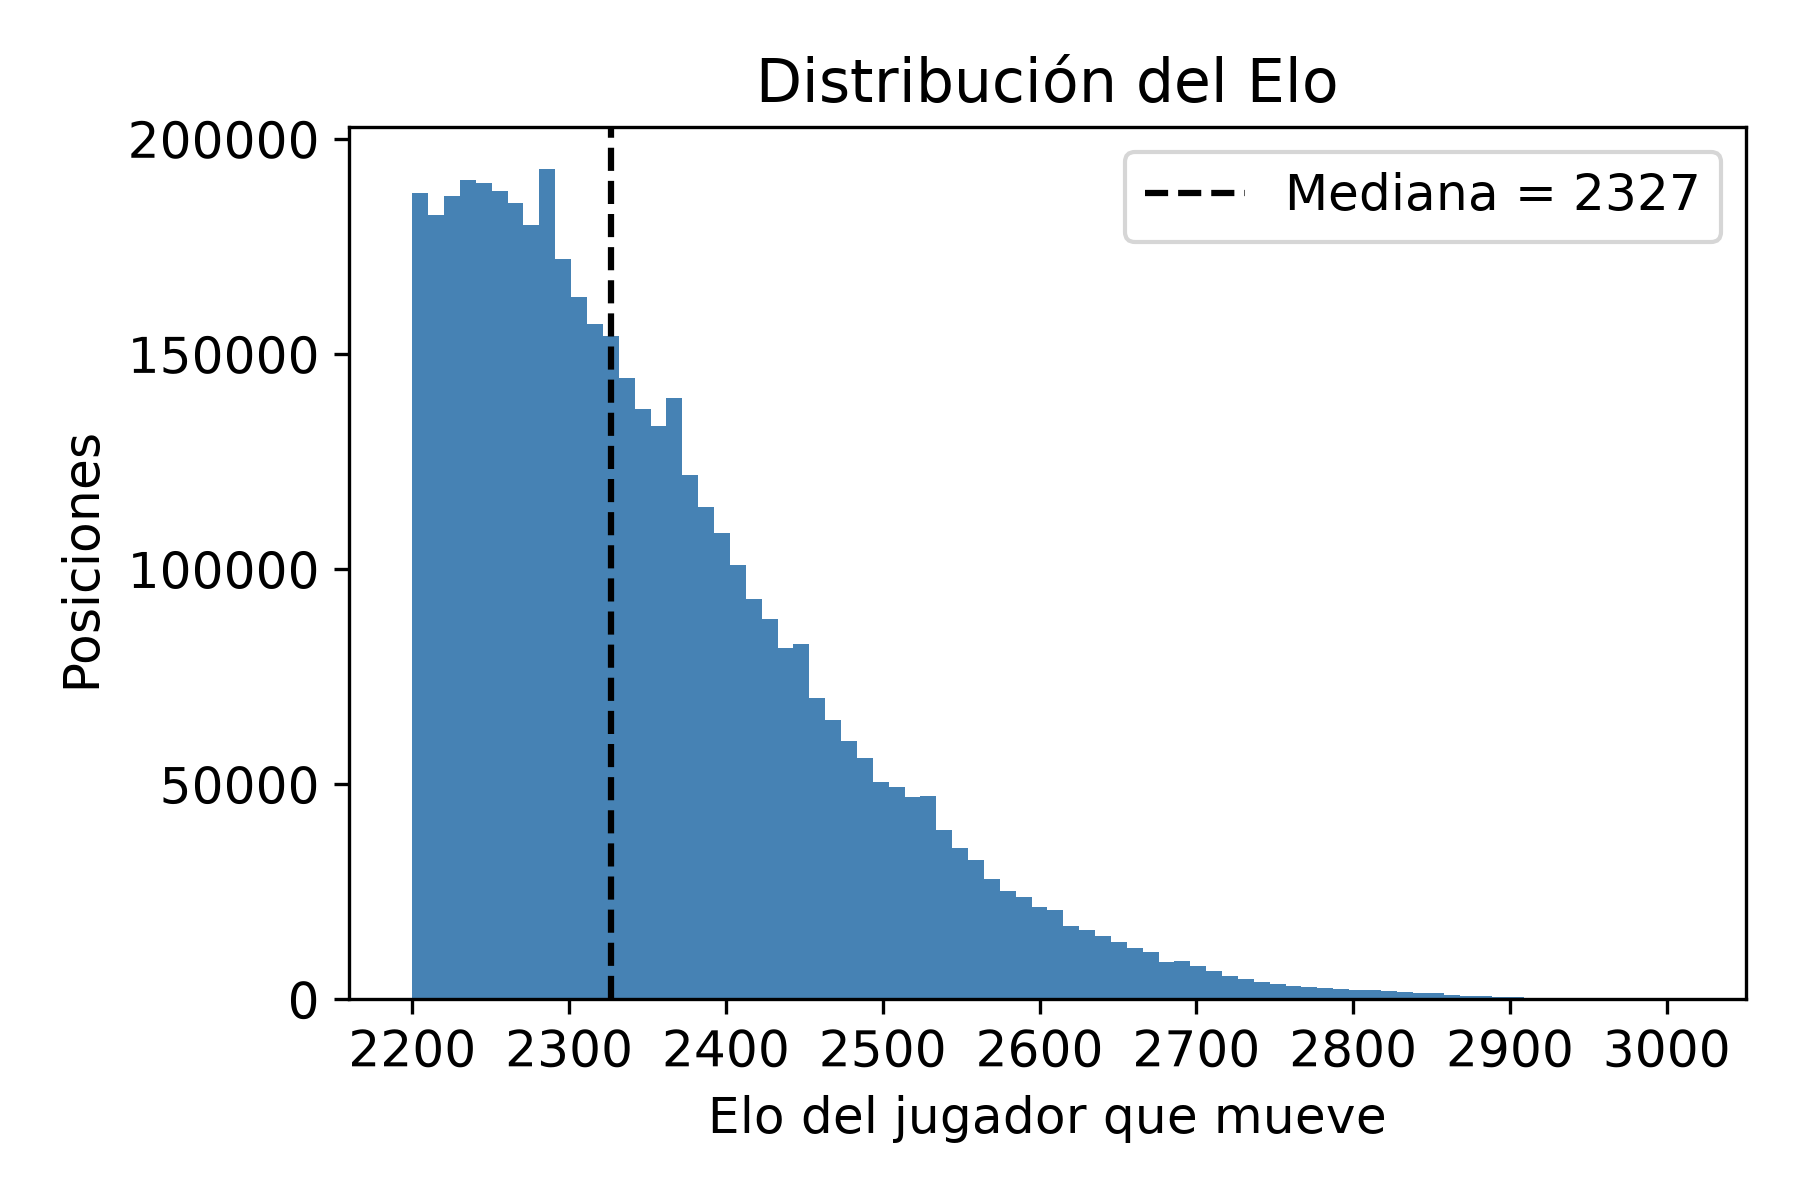
\includegraphics[width=\columnwidth]{figuras/eda_elo.png}
	\caption{Elo del jugador que mueve, ya sin las partidas de cuentas BOT.}
	\label{fig:eda-elo}
\end{figure}

\subsection{Momento de la partida y fases}

Las posiciones se concentran en los primeros \textit{plies} y su frecuencia baja conforme avanza la partida, porque muchas partidas terminan antes (figura~\ref{fig:eda-ply}); el \textit{ply} promedio es 39.1. El 82.9\% de las posiciones ocurre después del \textit{ply} 10.
\newline
Para analizar los resultados por fase definí tres grupos. El \textbf{final} son las posiciones con 12 piezas o menos, contando a los reyes; la \textbf{apertura}, el resto de las posiciones antes del \textit{ply} 20 (diez jugadas de cada bando); y el \textbf{medio juego}, todo lo demás. Con esta definición, el 30.8\% de las posiciones es de apertura, el 60.1\% de medio juego y el 9.2\% de final (figura~\ref{fig:eda-fases}). Como el final tiene pocas posiciones, sus resultados tendrán más incertidumbre.

\begin{figure}[H]
	\centering
	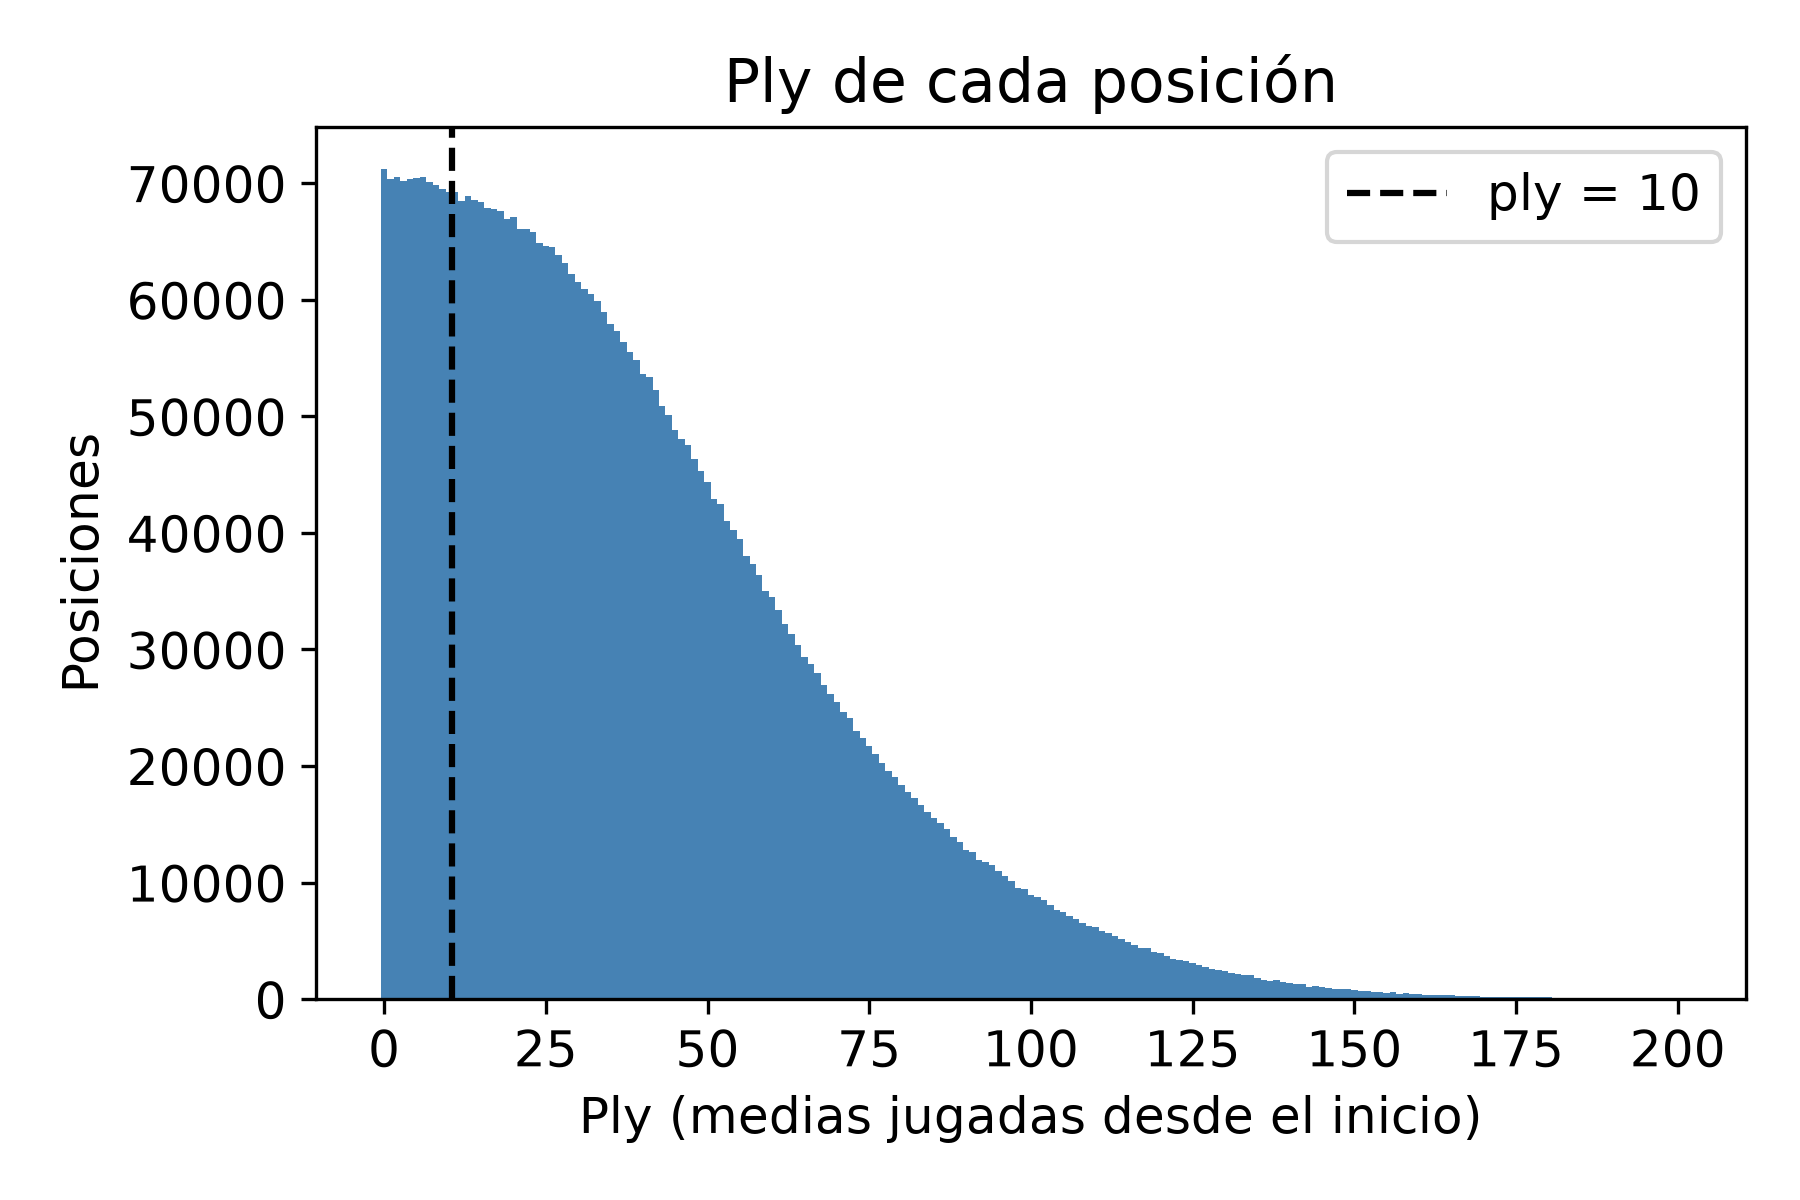
\includegraphics[width=\columnwidth]{figuras/eda_ply.png}
	\caption{\textit{Ply} en el que ocurre cada posición muestreada.}
	\label{fig:eda-ply}
\end{figure}

\begin{figure}[H]
	\centering
	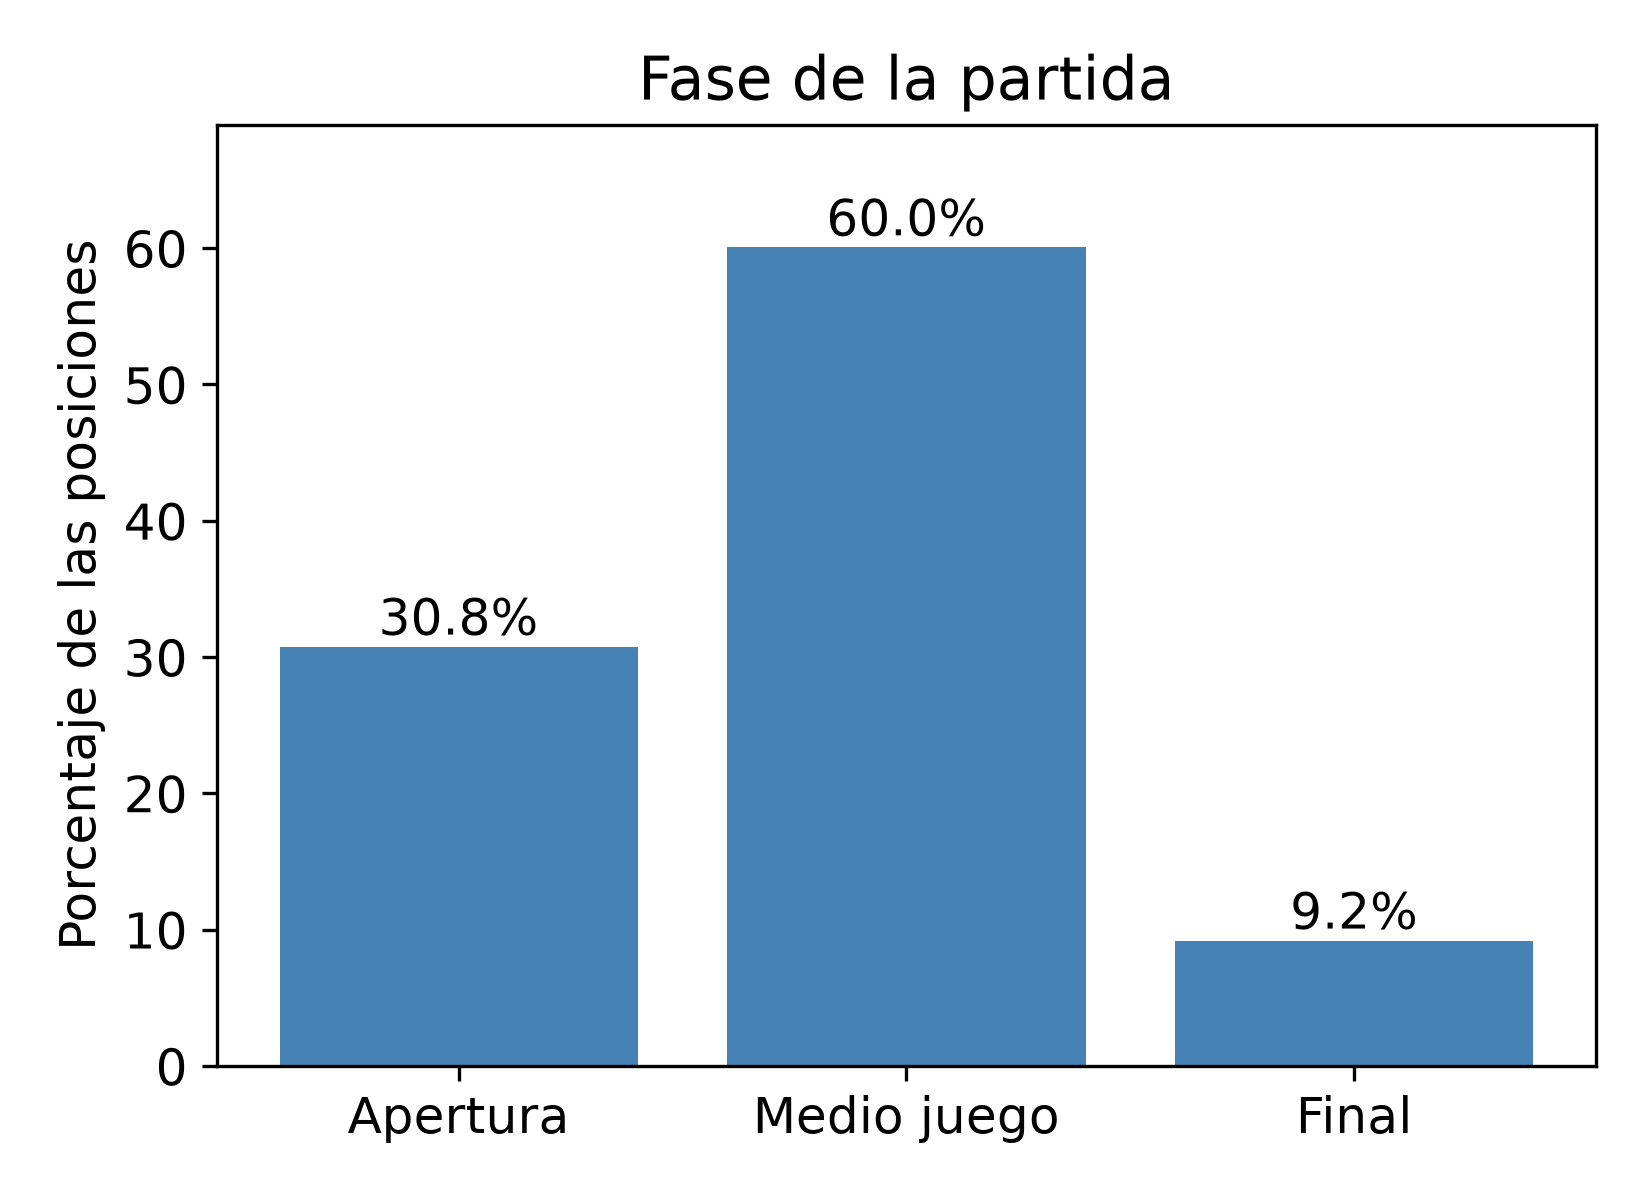
\includegraphics[width=0.85\columnwidth]{figuras/eda_fases.png}
	\caption{Posiciones por fase de la partida.}
	\label{fig:eda-fases}
\end{figure}

\subsection{Jugadas legales y la línea base del azar}

Cada posición tiene en promedio \textbf{31.0 jugadas legales}, con un mínimo de 1 y un máximo de 100 (figura~\ref{fig:eda-legales}). El pico en 20 corresponde a la posición inicial y a otras posiciones de apertura muy parecidas. El 0.6\% de las posiciones tiene una sola jugada legal y el 4.0\%, cuatro o menos.
\newline
Si se elige una jugada legal al azar, se acierta el \textbf{5.4\%} de las veces en promedio. Es más que $1/31.0 \approx 3.2\%$ porque en las posiciones con pocas opciones, como las de jaque, el azar acierta mucho más. Esta es la primera línea base que el modelo debe superar.

\begin{figure*}[t]
	\centering
	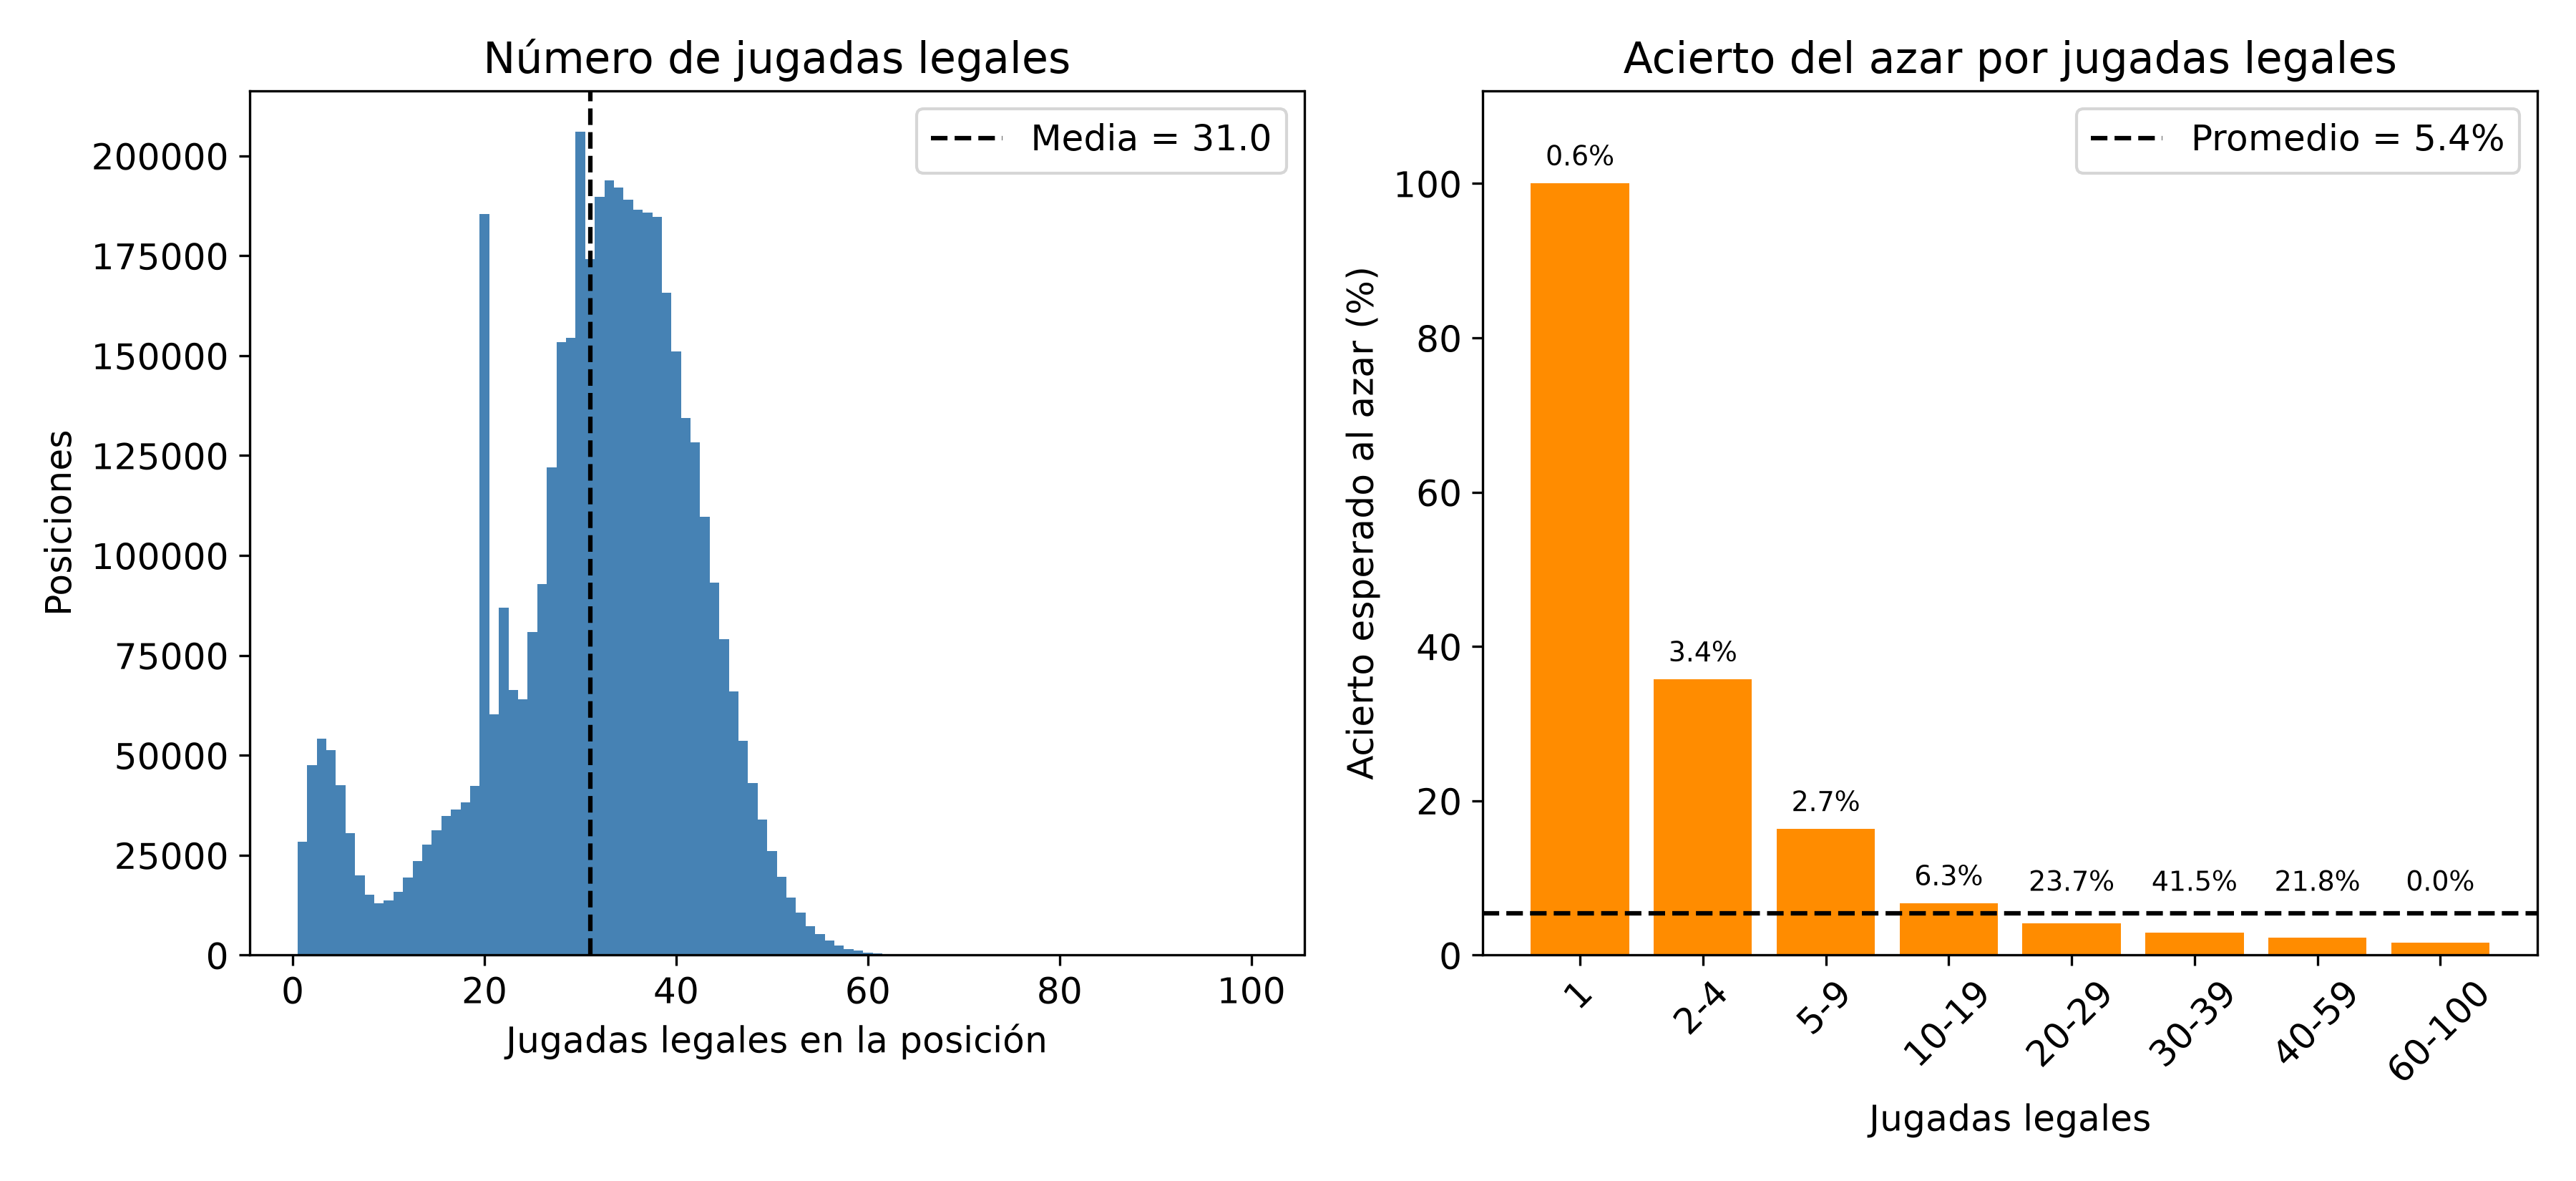
\includegraphics[width=\textwidth]{figuras/eda_jugadas_legales.png}
	\caption{Izquierda: número de jugadas legales por posición. Derecha: acierto esperado al elegir una jugada legal al azar, por intervalo; encima de cada barra, el porcentaje de posiciones del intervalo.}
	\label{fig:eda-legales}
\end{figure*}

\subsection{Las jugadas: clases, piezas y capturas}

Solo aparecen 1,792 de las 4,096 clases posibles, porque muchas combinaciones de origen y destino no corresponden al movimiento de ninguna pieza. Además, las clases que sí aparecen están muy desbalanceadas. La figura~\ref{fig:eda-clases} ordena las jugadas de la más a la menos común y muestra qué porcentaje del total se acumula: las 74 jugadas más comunes ya son la mitad de todas las jugadas del conjunto, 348 son el 80\% y 989 el 95\%. Las otras 803 juntas apenas suman el 5\% restante. Esto significa que el modelo verá muchísimos ejemplos de unas pocas jugadas y muy pocos del resto.

\begin{figure}[H]
	\centering
	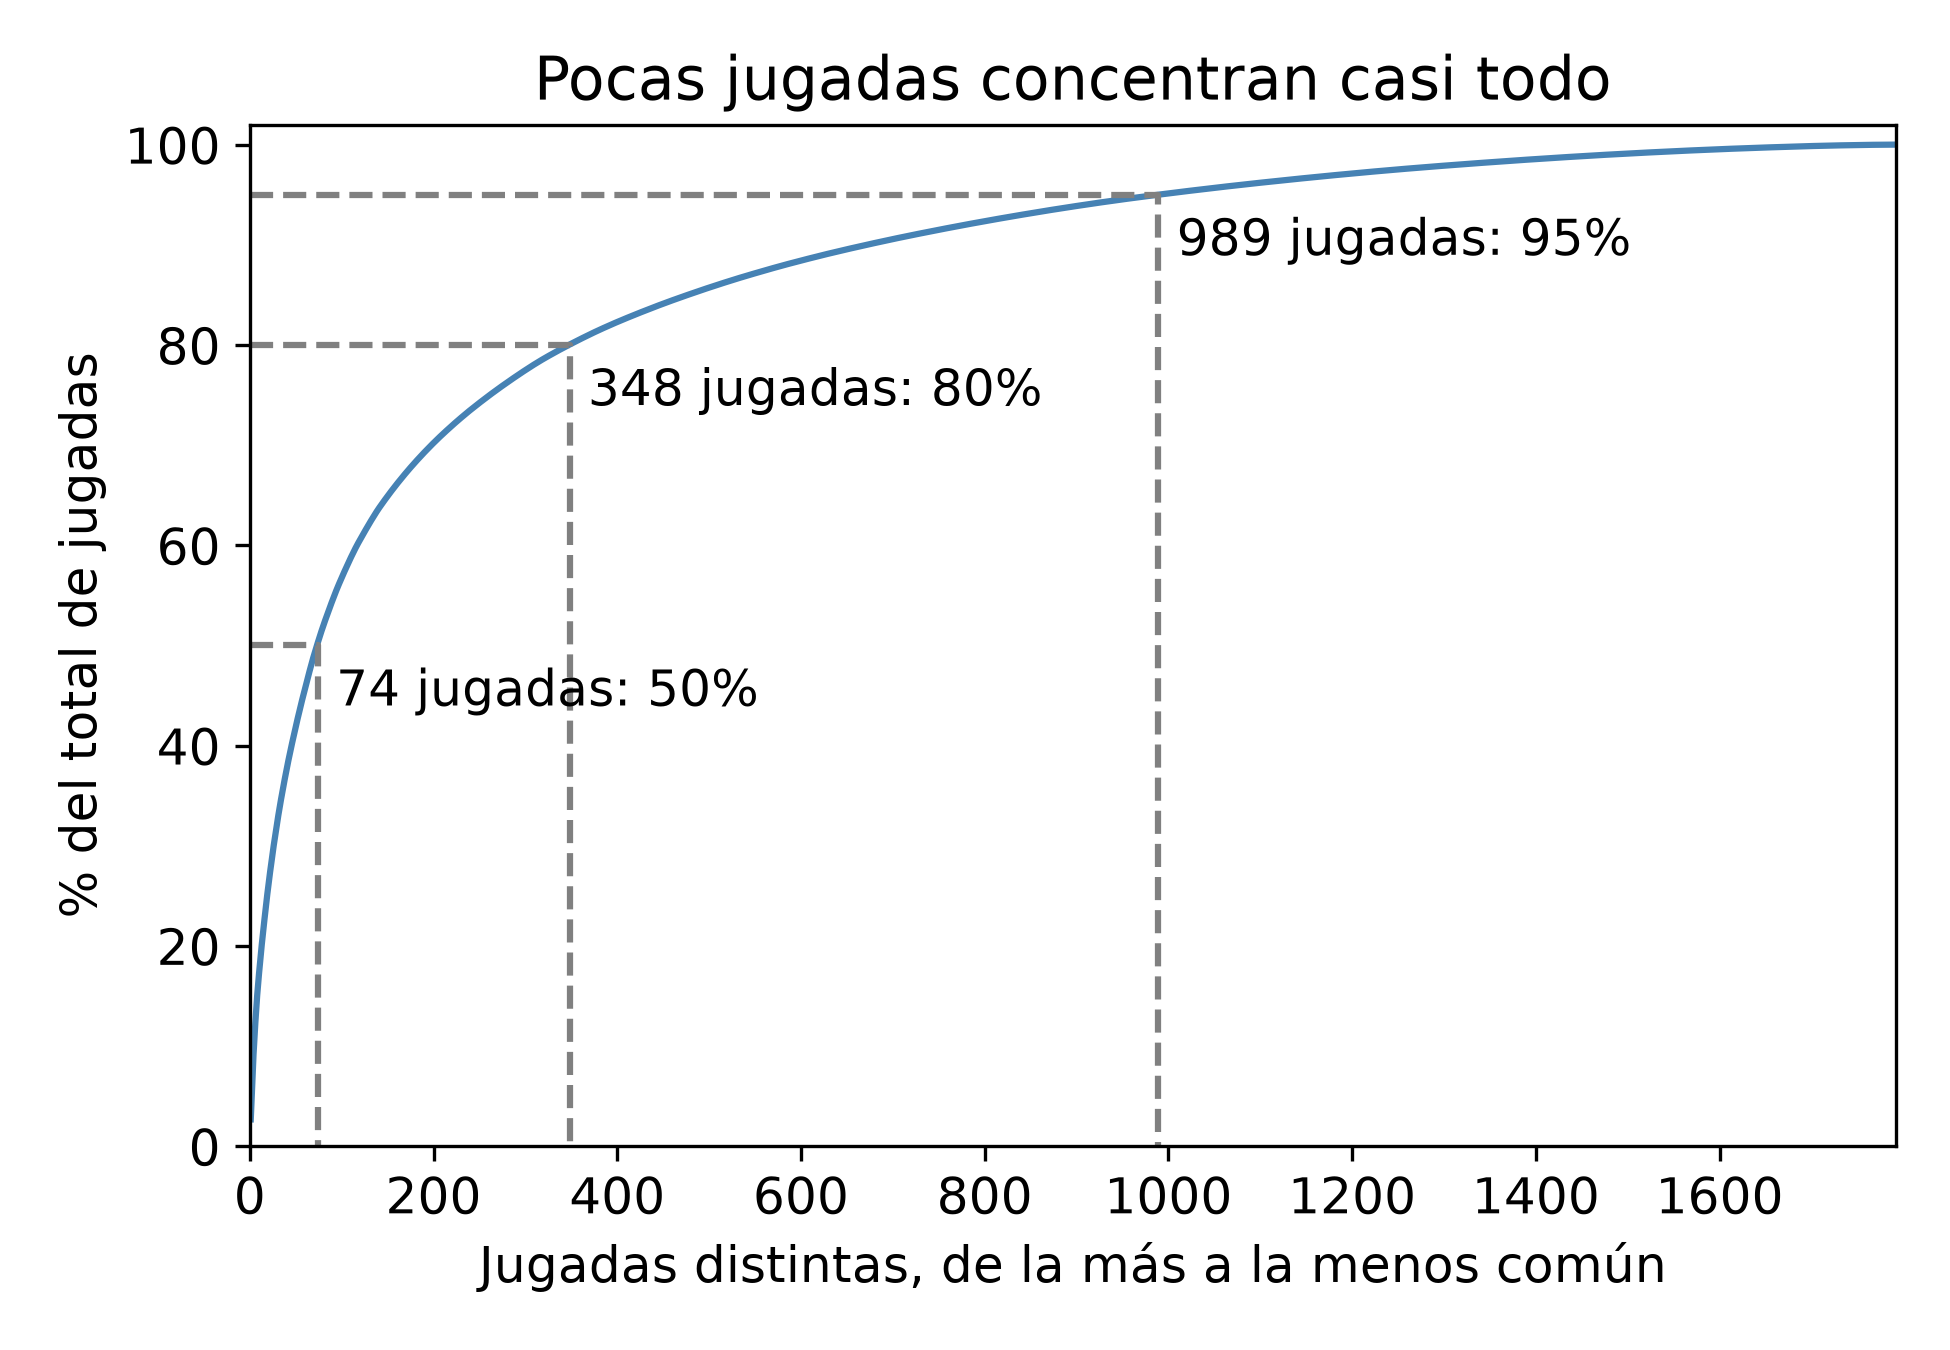
\includegraphics[width=\columnwidth]{figuras/eda_frecuencia_clases.png}
	\caption{Porcentaje acumulado de jugadas al sumar las clases de la más a la menos común. Las líneas punteadas marcan cuántas clases hacen falta para cubrir el 50\%, el 80\% y el 95\% de las jugadas.}
	\label{fig:eda-clases}
\end{figure}

La pieza que más se mueve es el peón (29.2\%), seguida del caballo (18.4\%) y el alfil (15.6\%); la torre, la dama y el rey se mueven entre el 11.2\% y el 13.9\% de las veces (figura~\ref{fig:eda-piezas}).
\newline
El 22.3\% de las jugadas son capturas (figura~\ref{fig:eda-capturas}). En el 75.7\% de las posiciones hay al menos una captura disponible, pero solo en el 25.0\% de ellas se juega la captura de mayor valor. Por eso espero que la línea base de «capturar la pieza más valiosa» sea débil: la mayoría de las veces los jugadores no capturan aunque puedan.

\begin{figure}[H]
	\centering
	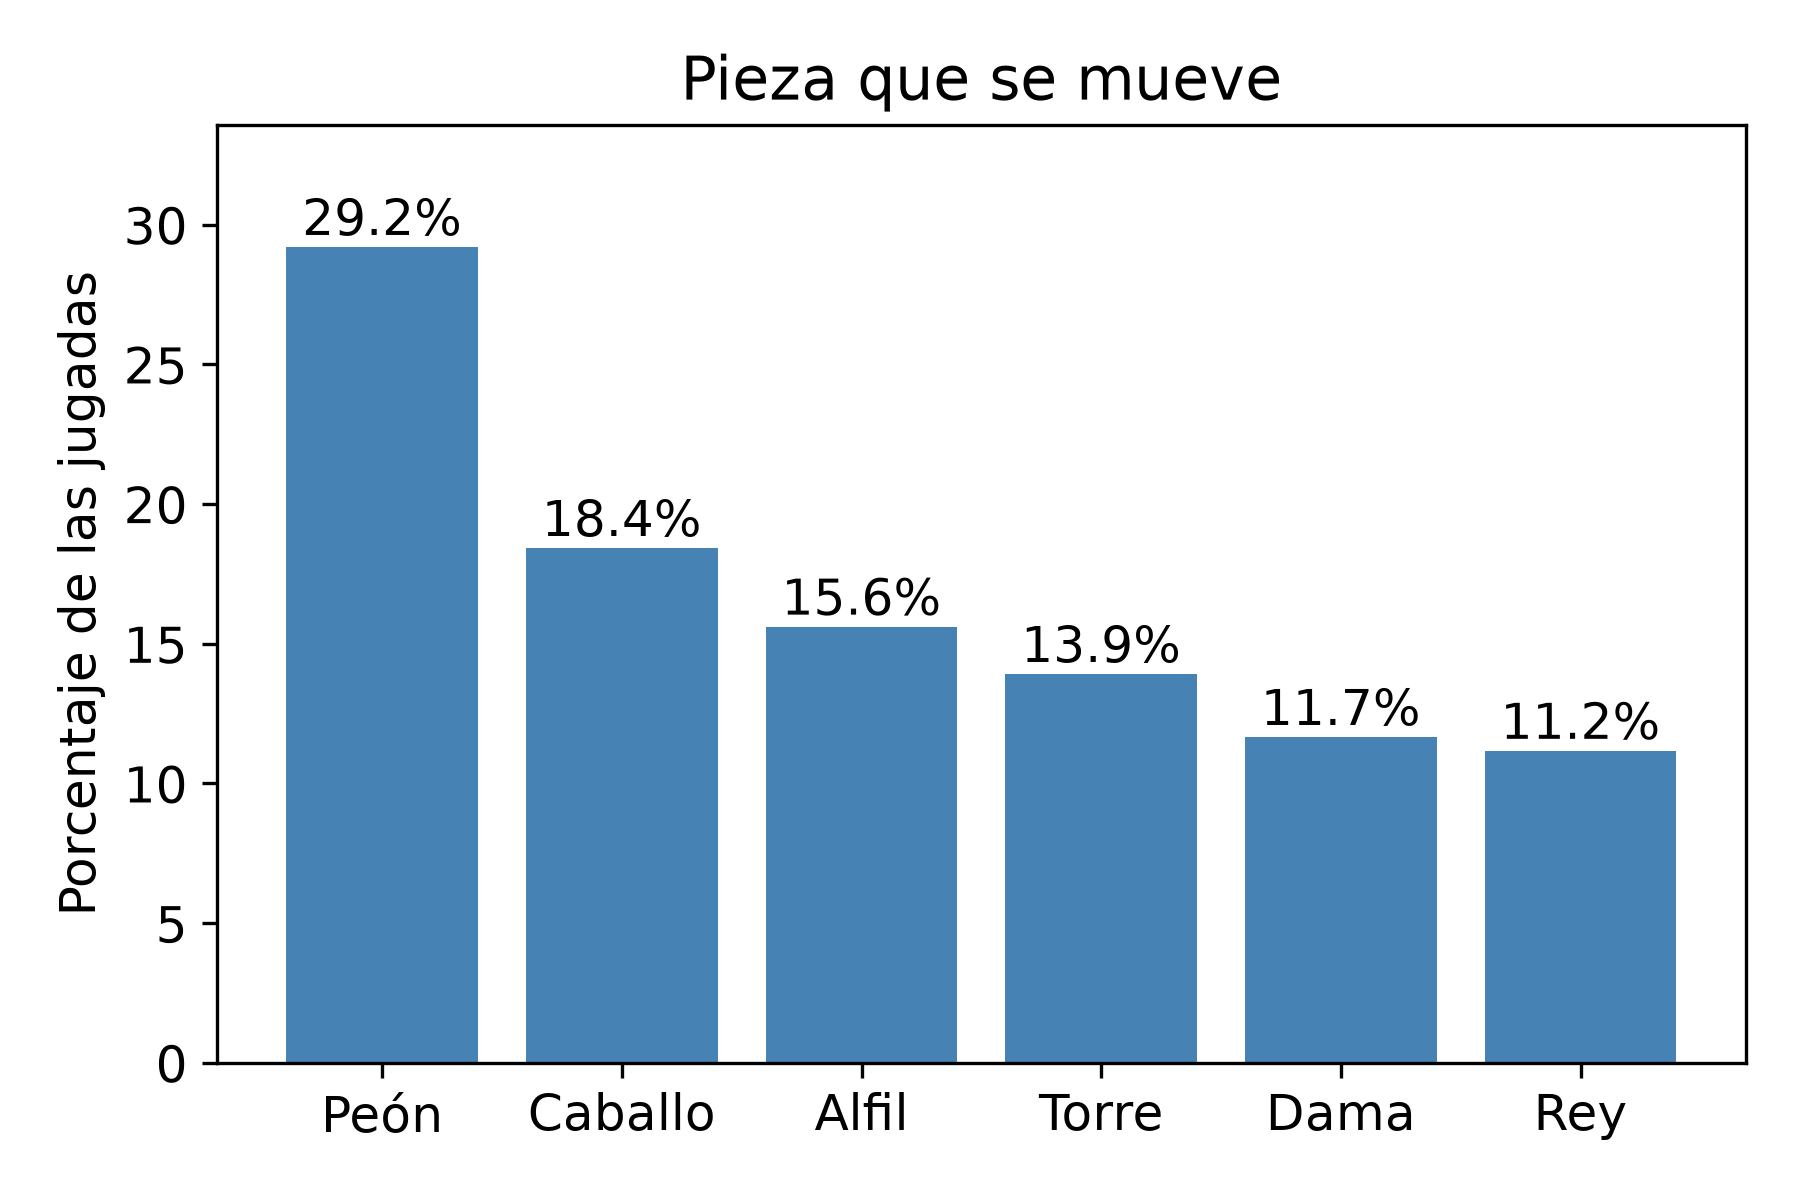
\includegraphics[width=0.85\columnwidth]{figuras/eda_pieza_movida.png}
	\caption{Tipo de pieza que se mueve en cada jugada.}
	\label{fig:eda-piezas}
\end{figure}

\begin{figure}[H]
	\centering
	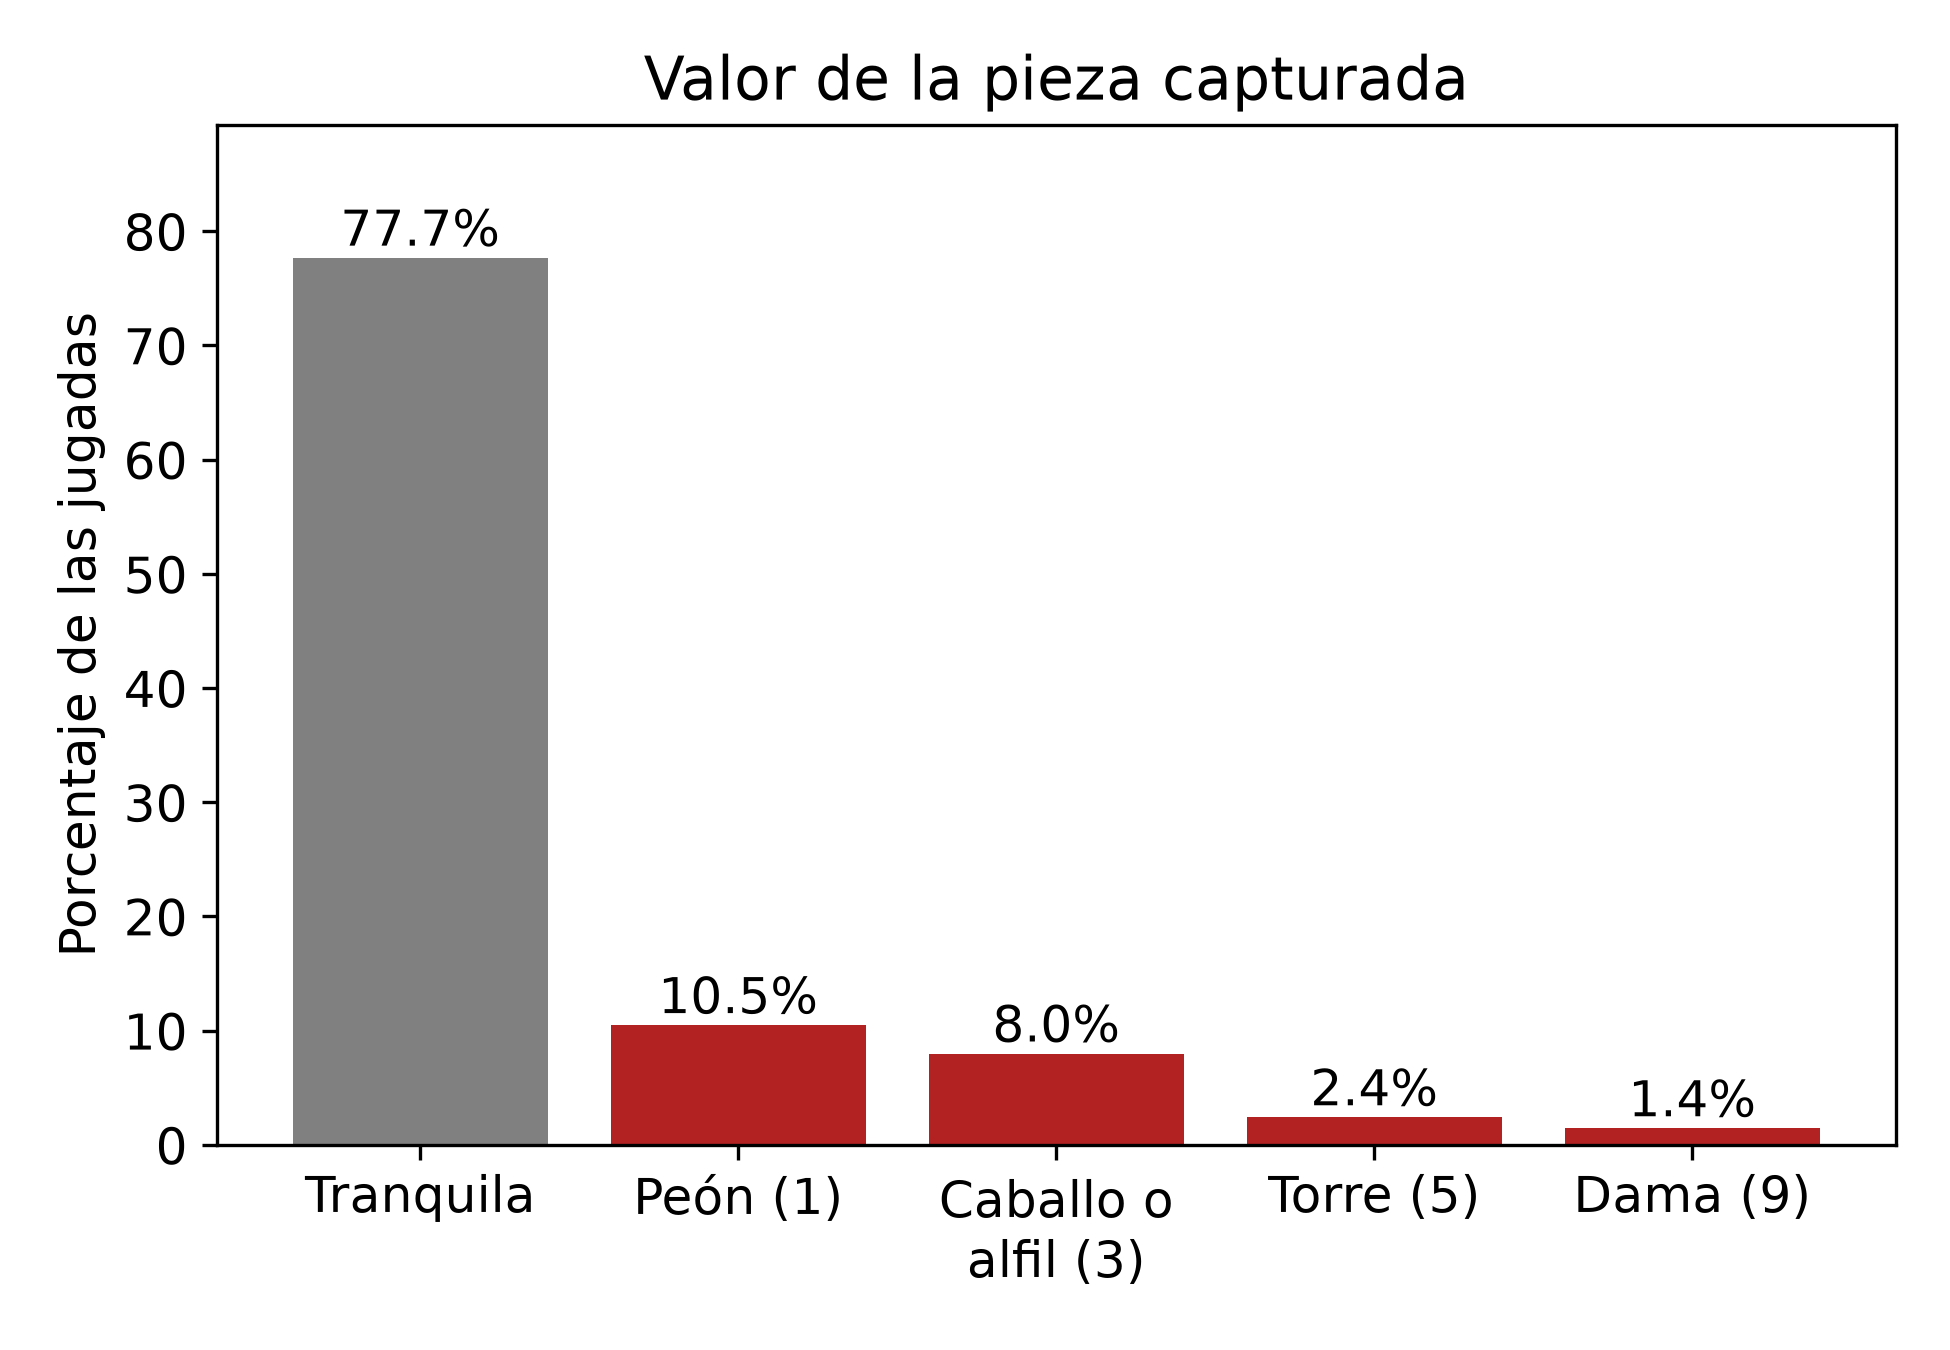
\includegraphics[width=0.85\columnwidth]{figuras/eda_capturas.png}
	\caption{Jugadas tranquilas y capturas, según el valor de la pieza capturada.}
	\label{fig:eda-capturas}
\end{figure}

\subsection{Posiciones que se repiten entre partidas}

Como incluí las aperturas, quise saber cuántas posiciones aparecen idénticas (mismas piezas, derechos de enroque y captura al paso) en dos o más partidas distintas. Se repiten porque muchos jugadores juegan las mismas aperturas, y eso significa que una parte de lo que aprenda el modelo en esas posiciones puede ser memoria.
\newline
El 21.6\% de las posiciones aparece en al menos dos partidas. Casi todas son de apertura: ahí se repite el 68.0\% de las posiciones, mientras que en el resto de la partida solo el 1.0\%. Por \textit{ply}, la posición inicial se repite siempre, en el \textit{ply} 4 el 98.6\%, en el \textit{ply} 10 el 72.1\%, en el \textit{ply} 16 el 28.7\% y desde el \textit{ply} 26 menos del 2\% (figura~\ref{fig:eda-repetidas}). Las partidas de nivel alto siguen caminos conocidos durante más jugadas, probablemente porque estos jugadores conocen más teoría de aperturas: en el mes de 2013, en el \textit{ply} 10 solo se repetía el 29.8\% de las posiciones.
\newline
En esas posiciones repetidas, la jugada más frecuente se elige el 62.1\% de las veces. Es decir, en una misma posición distintos jugadores eligen jugadas distintas, y ningún modelo que solo vea el tablero puede acertar todas: en estas posiciones, el acierto \textit{top-1} tiene un techo cercano al 62\%. En la posición inicial el techo es todavía más bajo, del 48.1\%, porque los jugadores reparten su primera jugada entre 1.e4 (48.1\%), 1.d4 (32.2\%), 1.\,Nf3 (8.4\%) y 1.c4 (5.9\%), entre otras.

\begin{figure}[H]
	\centering
	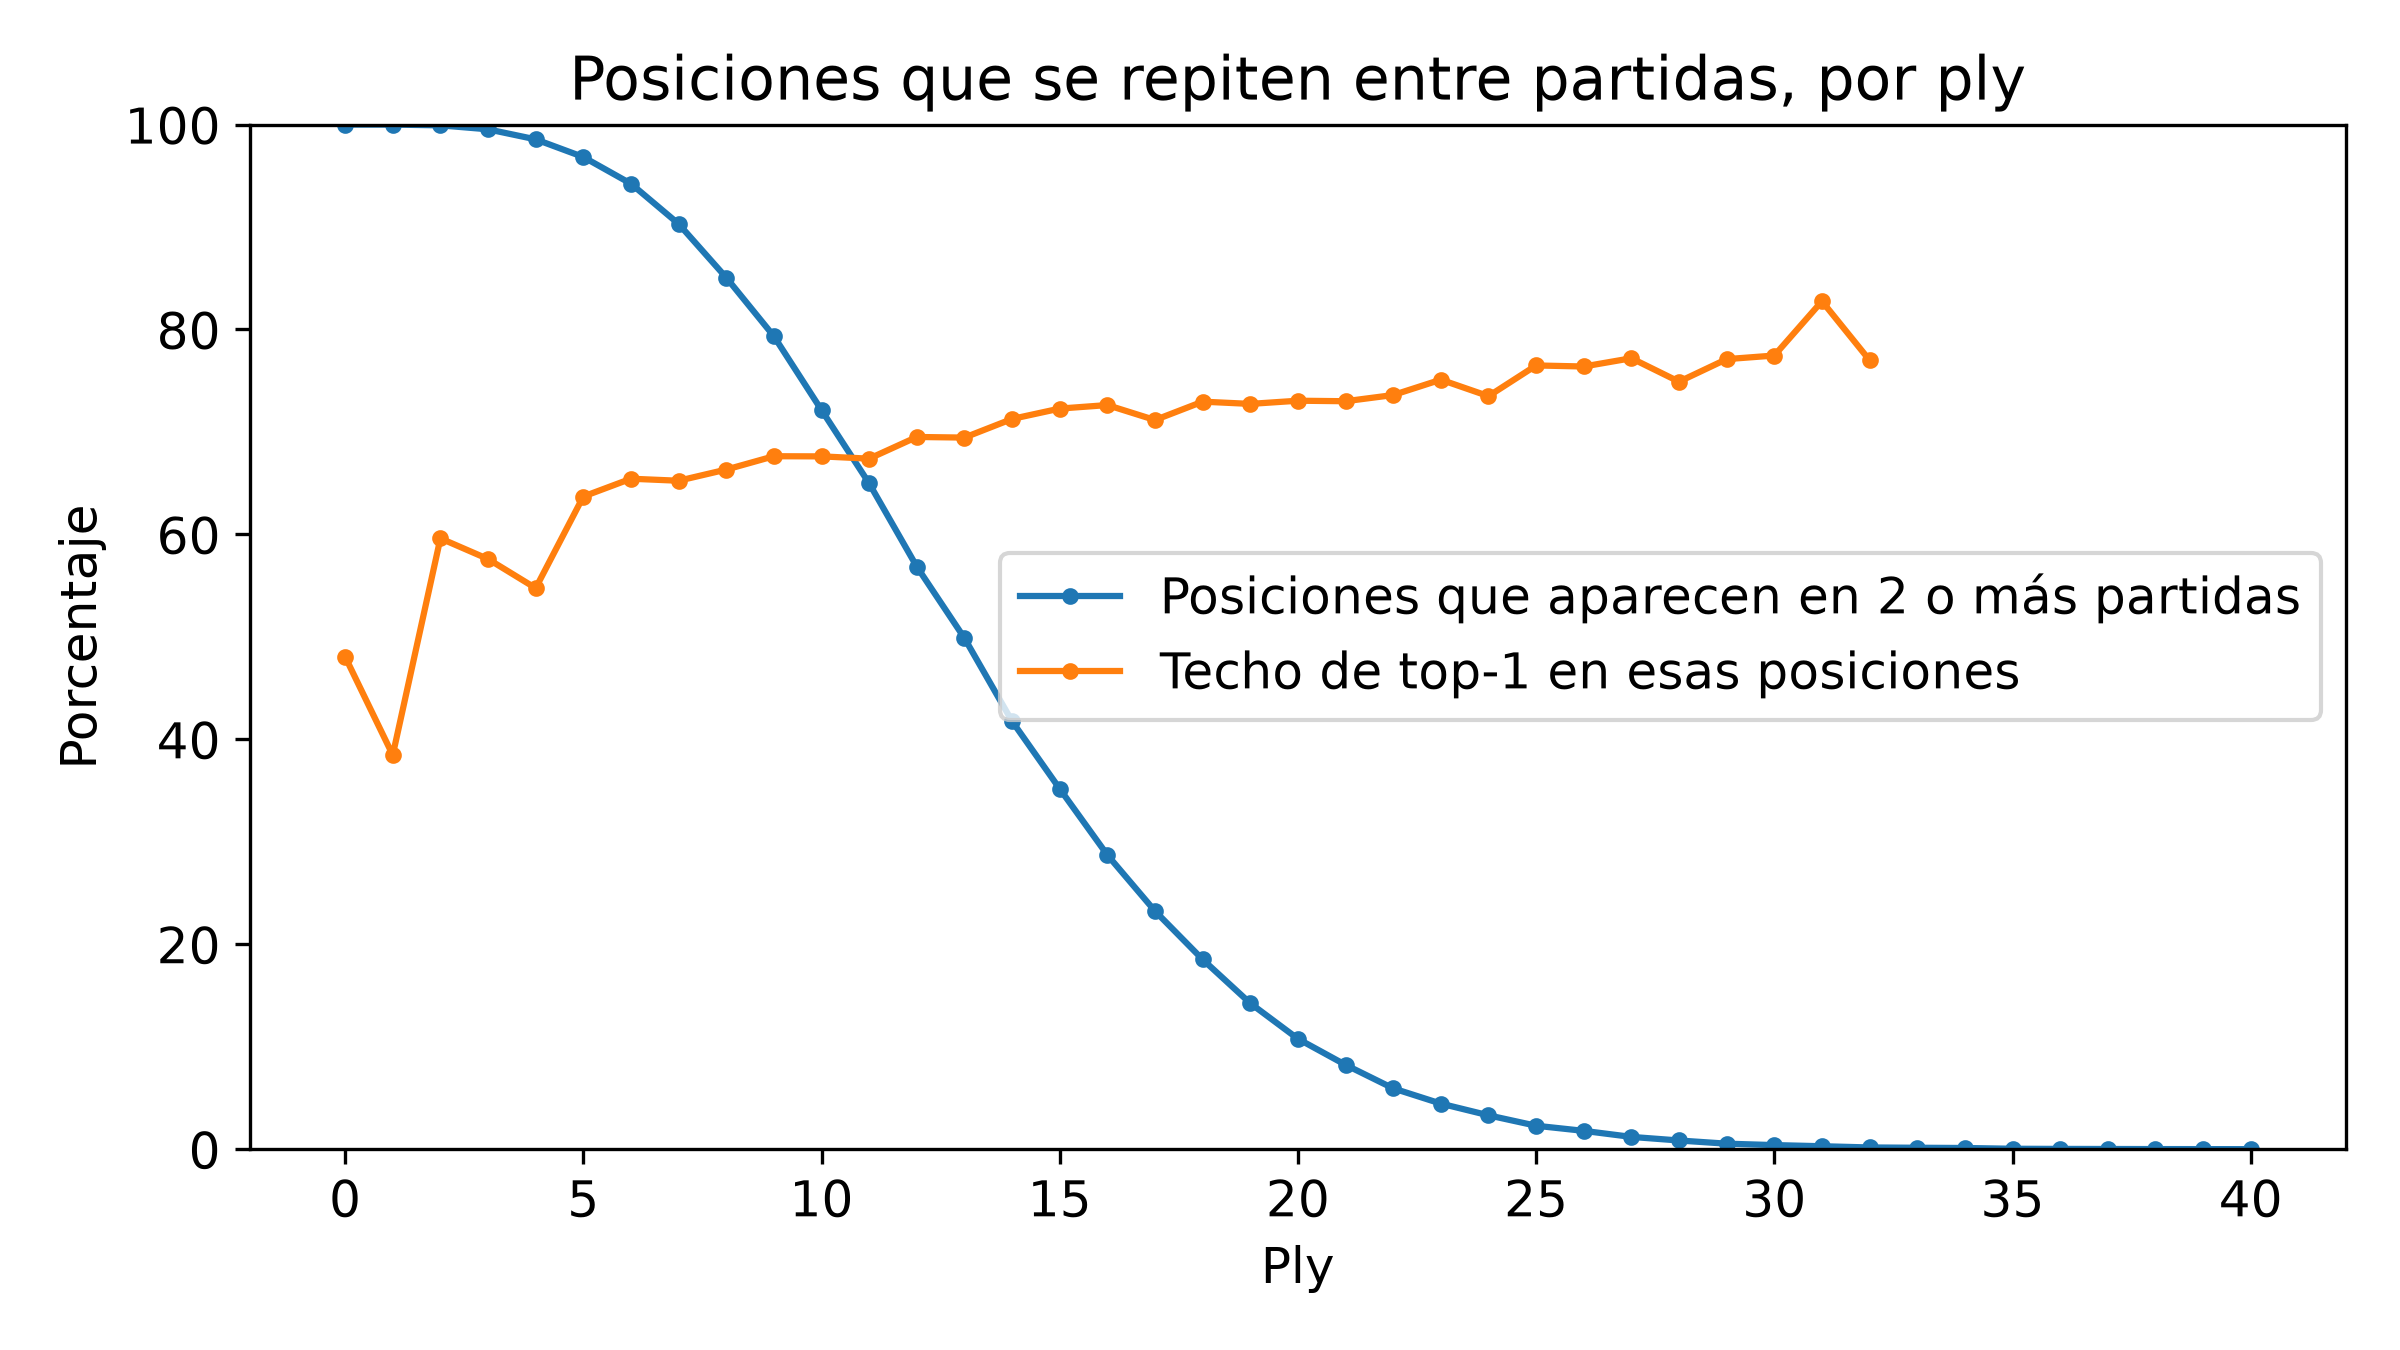
\includegraphics[width=\columnwidth]{figuras/eda_posiciones_repetidas.png}
	\caption{Por \textit{ply}: porcentaje de posiciones que aparecen en dos o más partidas y techo del acierto \textit{top-1} en esas posiciones. Solo se grafican los \textit{plies} con al menos 100 posiciones.}
	\label{fig:eda-repetidas}
\end{figure}

\subsection{Conclusiones del análisis}

\begin{itemize}[leftmargin=*]
	\item Usé solo partidas entre jugadores humanos con un Elo de 2,200 o más; las cuentas BOT quedaron fuera.
	\item Las fases quedan definidas por \textit{ply} (apertura antes del 20) y por número de piezas (final con 12 o menos), y reportaré los resultados de cada una por separado.
	\item El modelo tiene que superar al azar (5.4\%) en todo el conjunto.
	\item Más de dos tercios de las posiciones de apertura se repiten entre partidas, así que en la apertura también lo compararé con el «libro» (sección~\ref{sec:lineas-base}), que solo usa memoria.
	\item En las posiciones repetidas, el acierto \textit{top-1} no puede pasar de alrededor del 62\%, porque los jugadores no coinciden entre sí.
	\item La cola larga de clases y el bajo porcentaje de capturas de mayor valor indican que el modelo tendrá que aprender jugadas poco frecuentes y que una regla sencilla no bastará.
\end{itemize}

% =====================================================================
\section{Metodología de evaluación}

\subsection{Durante el entrenamiento}

La red se entrena con la entropía cruzada categórica (\textit{sparse categorical crossentropy}), la pérdida para clasificación cuando las etiquetas son enteros. En cada época registro la pérdida y la precisión en entrenamiento y validación. Con \textit{ModelCheckpoint} guardo el modelo de menor pérdida en validación, de modo que el número de épocas no tiene que adivinarse de antemano.

\subsection{Precisión \textit{top-k}}

Para cada posición el modelo da una probabilidad a cada una de las 4,096 jugadas posibles. Primero descarto las jugadas ilegales, porque en una partida nunca podrían elegirse, y ordeno las legales de la más a la menos probable. Después busco en qué lugar de esa lista quedó la jugada que realmente se jugó. La precisión \textit{top-k} es el porcentaje de posiciones en las que la jugada real quedó entre las $k$ primeras; con $k = 1$ es la exactitud usual de un clasificador.
\newline
Por ejemplo, si en la posición inicial el modelo ordena 1.e4 (40\%), 1.d4 (30\%) y 1.\,Nf3 (10\%), y el jugador eligió 1.d4, la jugada real quedó en segundo lugar: la posición cuenta como fallo en \textit{top-1} y como acierto en \textit{top-3} y \textit{top-5}.
\newline
Elegí esta métrica porque es la que usan los trabajos que, como este, buscan predecir la jugada de una persona. McIlroy-Young et al.~\cite{mcilroyyoung2020} miden la precisión de coincidencia con la jugada humana (\textit{move-matching accuracy}), que es el \textit{top-1}, y al evaluar solo consideran las jugadas legales que produce la red. Ellos mismos señalan su límite: como jugadores distintos eligen jugadas distintas en la misma posición, ningún modelo puede coincidir con todos. Por eso también reporto \textit{top-3} y \textit{top-5}, como hacen Soldera y Pedrini~\cite{soldera2026} con su lista ordenada de jugadas candidatas (ellos llegan a \textit{top-3}): si la jugada humana queda en segundo o tercer lugar, el modelo la consideró aunque no la eligiera, y eso no es lo mismo que haberla ignorado. En este conjunto el problema es concreto, porque en las posiciones repetidas la jugada más común solo se elige el 62.1\% de las veces (sección~\ref{sec:eda}).
\newline
Como la red se entrena sin la restricción de legalidad, también mido qué porcentaje de sus primeras opciones es ilegal, para saber si aprendió las reglas. Las líneas base de la sección~\ref{sec:lineas-base} se evalúan exactamente igual: cada una ordena las jugadas legales con su propia regla y se mide en qué lugar quedó la jugada real.
\newline
La métrica principal se calcula sobre \textbf{todas} las posiciones, incluidas las de apertura. Además la desgloso por fase (apertura, medio juego y final). Solo como referencia, para compararme con el protocolo de Maia, también la calculo sin los primeros 10 \textit{plies}.

\subsection{Conjuntos de entrenamiento y validación}

Antes de comparar nada revisé que entrenamiento y validación se parecieran. Las distribuciones del Elo, del \textit{ply} y de las fases prácticamente se enciman (figura~\ref{fig:train-val}), así que la división por partida no dejó a ninguno de los dos conjuntos con jugadores, momentos de la partida o fases distintos. El conjunto de prueba no lo reviso hasta la evaluación final.

\begin{figure*}[t]
	\centering
	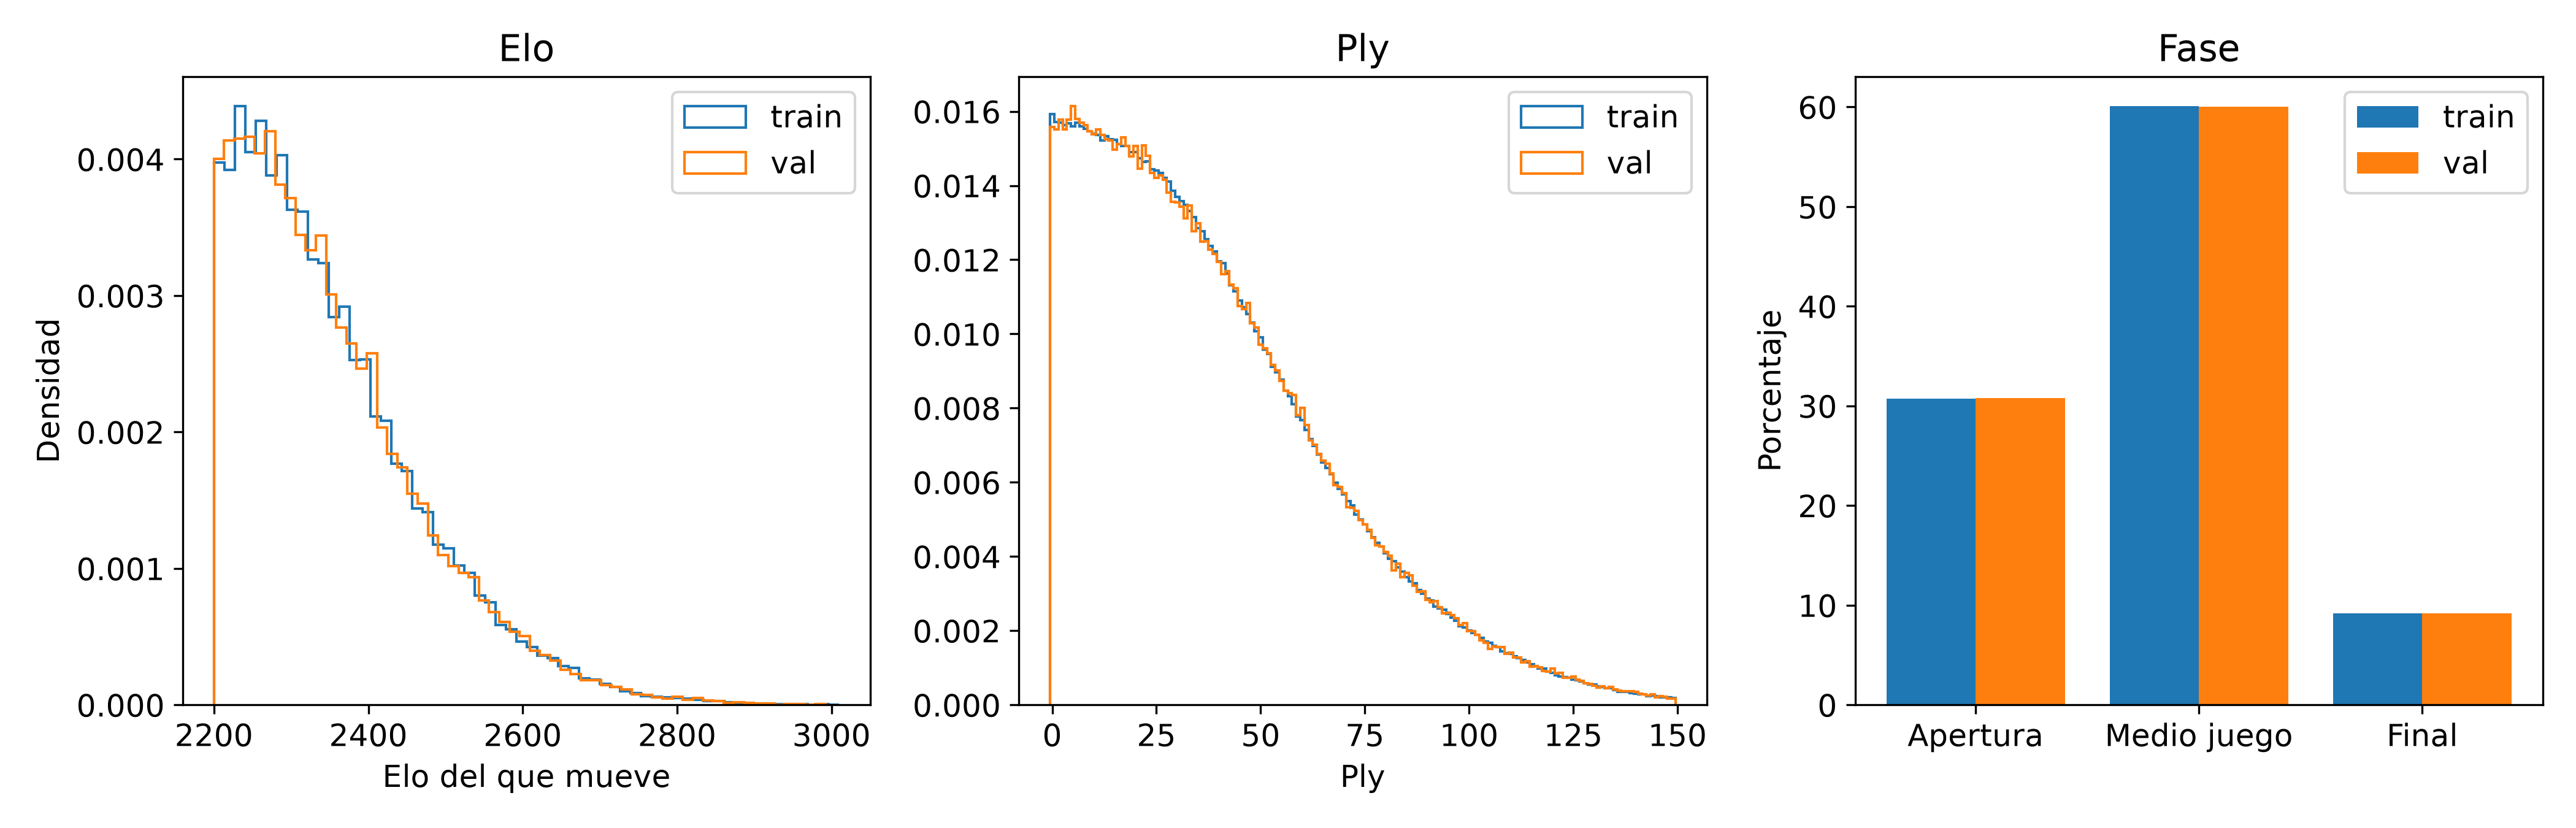
\includegraphics[width=\textwidth]{figuras/comparacion_train_val.png}
	\caption{Elo del jugador que mueve, \textit{ply} y fase de la partida en entrenamiento (\textit{train}) y validación (\textit{val}).}
	\label{fig:train-val}
\end{figure*}

Aunque ninguna partida está en los dos conjuntos, el 21.0\% de las posiciones de validación aparece idéntica en entrenamiento. Casi todas son de apertura: ahí está repetido el 66.3\% de las posiciones, contra el 0.9\% en el medio juego y el 0.7\% en el final. No es una fuga de datos, porque son posiciones distintas de partidas distintas que coinciden porque los jugadores repiten las mismas aperturas; pero en ellas se puede acertar solo con memoria, y eso es lo que mide la línea base del «libro».

\subsection{Líneas base}
\label{sec:lineas-base}

Todas las métricas se comparan con cuatro líneas base calculadas con los mismos datos:
\begin{enumerate}[leftmargin=*]
	\item una jugada legal al azar;
	\item la jugada legal más frecuente en el conjunto de entrenamiento;
	\item la captura de mayor valor y, si no hay capturas, una jugada legal al azar;
	\item un «libro»: si la posición exacta aparece en entrenamiento, la jugada que más se jugó en ella y, si no aparece, la jugada legal más frecuente. Esta línea base mide cuánto se puede acertar solo con memoria, sobre todo en la apertura, donde las mismas posiciones se repiten en muchas partidas.
\end{enumerate}
Cuando dos jugadas empatan, por ejemplo dos capturas del mismo valor, el orden entre ellas se decide al azar. La tabla~\ref{tab:lineas-base} muestra el acierto de cada línea base en las 450,591 posiciones de validación.

\begin{table*}[t]
	\centering
	\footnotesize
	\setlength{\tabcolsep}{4pt}
	\begin{tabular}{lrrrrrrr}
		\hline
		 & \multicolumn{3}{c}{Todas las posiciones} & \multicolumn{4}{c}{\textit{Top-1} por corte} \\
		Línea base & \textit{Top-1} & \textit{Top-3} & \textit{Top-5} & Apertura & Medio juego & Final & \shortstack[r]{Sin los primeros\\10 \textit{plies}} \\
		\hline
		Azar & 5.4 & 14.4 & 21.7 & 3.6 & 5.3 & 12.1 & 5.7 \\
		Más frecuente & 11.0 & 22.9 & 33.0 & 18.7 & 6.3 & 15.4 & 9.3 \\
		Captura de mayor valor & 15.6 & 29.0 & 36.0 & 10.3 & \textbf{17.5} & \textbf{20.5} & \textbf{16.7} \\
		Libro & \textbf{18.7} & \textbf{29.6} & \textbf{37.8} & \textbf{42.8} & 6.7 & 15.6 & 12.3 \\
		\hline
		Posiciones & \multicolumn{3}{r}{450,591} & 138,733 & 270,364 & 41,494 & 380,124 \\
		\hline
	\end{tabular}
	\caption{Acierto de las líneas base en validación (\%). En negritas, la mejor de cada columna.}
	\label{tab:lineas-base}
\end{table*}

El «libro» es la mejor línea base en el conjunto completo (18.7\% \textit{top-1}), pero casi todo su acierto viene de la apertura, donde llega al 42.8\%. Fuera de ella las posiciones casi nunca están en entrenamiento, así que termina eligiendo la jugada más frecuente y apenas supera al azar en el medio juego.
\newline
Contra lo que esperaba en el análisis exploratorio, capturar la pieza más valiosa es la mejor regla en el medio juego (17.5\%), en el final (20.5\%) y sin los primeros 10 \textit{plies} (16.7\%). Aunque los jugadores solo eligen la captura de mayor valor en una de cada cuatro posiciones con capturas, ninguna de las otras reglas se acerca a eso fuera de la apertura.
\newline
Con esto, el modelo tiene dos referencias claras: superar al «libro» en la apertura, donde se puede acertar de memoria, y superar a la captura de mayor valor en el resto de la partida, donde tiene que entender la posición.

% =====================================================================
\onecolumn
\section{Códigos}

Todos los códigos están en \url{https://github.com/TheSimpleMau/Portafolio-Implementacion-Deeplearning}. Aquí se incluyen los módulos principales hasta el momento.

Codificación del tablero y de las jugadas.
\lstinputlisting[style=pythonish]{../model/preprocessing.py}

\newpage
Proceso de ETL.
\lstinputlisting[style=pythonish]{../model/etlProcess.py}

\newpage
Análisis exploratorio.
\lstinputlisting[style=pythonish]{../model/eda.py}

\newpage
Gráficas.
\lstinputlisting[style=pythonish]{../model/plotUtil.py}

\newpage
Evaluación y líneas base.
\lstinputlisting[style=pythonish]{../model/evaluation.py}

\clearpage
\printbibliography[heading=bibintoc, title={Referencias}]

\end{document}
